\documentclass[11pt]{article}
\usepackage[utf8]{inputenc}
\usepackage{amsmath,amssymb,amsthm}
\usepackage{hyperref}
\usepackage[capitalise,noabbrev]{cleveref}
\usepackage{geometry}
\usepackage{booktabs}
\usepackage{graphicx}
\geometry{margin=1in}

% Theorem environments
\newtheorem{theorem}{Theorem}[section]
\newtheorem{proposition}[theorem]{Proposition}
\newtheorem{corollary}[theorem]{Corollary}
\newtheorem{lemma}[theorem]{Lemma}
\theoremstyle{definition}
\newtheorem{definition}[theorem]{Definition}
\newtheorem{conjecture}[theorem]{Conjecture}
\theoremstyle{remark}
\newtheorem{remark}[theorem]{Remark}

\title{Spectral Gap Selection of Lorentzian Signature\\
from Observer Fisher Information Geometry}

\author{Max Zhuravlev\thanks{Independent researcher. Email: \texttt{max@vibecodium.ai}}}

\date{February 2026}

\begin{document}

\maketitle

\begin{abstract}
We prove that Fisher information matrices of Ising-model observers on
sparse graphs select Lorentzian signature~$(1,n{-}1)$ through a spectral gap
mechanism. Given the weighting functional $W(q) = \beta_c(q) \cdot
L_{\mathrm{gap}}(q)$ for a sign assignment with $q$~negative entries,
we establish three main results (Theorems~A--C):
\textbf{(A)}~For any positive definite diagonal~$F$, $W(1) > W(q)$ for all
$q \geq 2$ (exact; subsumes tree graphs via the Tree Fisher Identity
$F = \operatorname{sech}^2(J) \cdot I$);
\textbf{(B)}~Lorentzian selection persists under near-diagonal perturbations
$F = D + \varepsilon E$ with explicit threshold
$\varepsilon_0 = d_{\min}/(2\Gamma(\kappa))$, $\Gamma(\kappa) = \sqrt{2\kappa} + \tfrac{1}{4}$;
\textbf{(C)}~the near-diagonal condition holds for bounded-degree graphs at
subcritical coupling $J < J_{\mathrm{crit}}(\Delta, g)$.
\textbf{Scope limitation (Ising-specific):} The Ising mechanism fails for regular grid
topologies at strong coupling ($J \geq 1$), with only 30--43\% Lorentzian
selection, confirming near-diagonality---not merely bounded degree---as the
structural prerequisite. However, this limitation is entirely specific to the
discrete $\mathbb{Z}_2$ symmetry: continuous $O(N \geq 2)$ spins achieve $100\%$
selection on all tested grids at all coupling strengths. Combined with the PSD obstruction ($M = F^2$ is always
positive semi-definite), these results identify the signed-edge construction
as the natural mechanism for Lorentzian signature selection.
\textbf{Universality:} The $O(n)$ Tree Fisher Identity extends to XY and
Heisenberg models, giving $W(1) > 0 = W(q \geq 2)$ unconditionally.
Ising observers on causal set Hasse diagrams (Bombelli--Sorkin sprinklings)
select Lorentzian at $94\%$ ($220/234$ configurations).
\textbf{O(N) hierarchy:} For continuous $O(N)$ spin models, selection robustness
increases monotonically with $N$: at $N \geq 10$, every one of $271$~atlas
graphs selects Lorentzian across all tested coupling strengths ($4{,}878$~configurations
total; $0/813$ failures for $N = 10$ and $N = 50$). The threshold $\beta_1^*(N)$
above which selection first fails grows with $N$ ($\beta_1^*(1) = 2$,
$\beta_1^*(4) = 6$, $\beta_1^*(10) > 15$); a fine-grained $N$-sweep
identifies $N^* = 5$ for the $n \leq 7$ atlas; an extended census on
$n = 7$--$12$ Ising-failing graphs ($\beta_1$ up to $41$) finds $N^* = 2$
for $86\%$ of $500$~tested, with rare $N^* \geq 4$ outliers (${\sim}6\%$)
exclusively at edge connectivity $\kappa = 2$ ($29/29$ cases).
Cross-validation on 50~dense counterexample graphs ($n \leq 12$,
$\beta_1 \geq 9$), 8~grid topologies up to $5 \times 6$ ($n = 30$),
and ${\sim}4{,}900$~random graphs $G(n,p)$ ($98$~cells, $n = 8$--$30$;
Ising three-regime phase diagram with dense rebound confirmed through
$n = 50$) confirms: $O(5)$ achieves $100\%$ Lorentzian on \emph{all} tested
topologies ($719$~graphs, $36$~cells), completely eliminating both the
Ising grid failure regime and the $G(n,p)$ non-Lorentzian valley.
\textbf{Graph-theoretic characterization:} An extended census of $18{,}040$~connected
graphs ($n \leq 12$) refines the edge connectivity picture: the original
conjecture ($\kappa(G) \leq 1 \Rightarrow$ always-Lorentzian) is refuted
by 200~counterexamples, all with $\beta_1 \geq 9$---dense components joined
by a bridge. The corrected conjecture, $\kappa(G) \leq 1$ AND $\beta_1(G) \leq 8$,
has zero counterexamples across all 18,040~graphs (accuracy $\approx 97.5\%$).
The sharp transition at $\kappa = 2$ (98.17\% always-L at $\kappa = 1$ vs.\ 5.46\%
at $\kappa = 2$) remains the strongest structural predictor.
The XY ($O(2)$) model on complete graphs $K_4$--$K_{25}$ achieves
$100\%$ Lorentzian ($352$~configurations), but $O(N)$ selection is
\emph{non-monotone}: $O(10)$ fails on $K_n$ for $n \geq 13$,
revealing an $O(2)$ sweet spot.
The XY model on $1025$~general
graphs ($2566$~configs) achieves $89.2\%$ always-Lorentzian, with the failure threshold
shifting from $\beta_1 \leq 1$ (Ising) to $\beta_1 \leq 3$ (XY, $100\%$).
\textbf{Multi-observer consensus:} Across $1{,}024$~graphs ($54{,}711$~observer
measurements), observers with local $\beta_{1,\mathrm{local}} \leq 1$ select
Lorentzian at $100\%$ ($14{,}793/14{,}793$) and agree on the timelike direction
with mean pairwise agreement $98.65\%$.
\textbf{$W(q)$ spectrum:} Testing $W(q)$ for \emph{all} $q$ on $258$~graphs
($774$~configurations) shows $q = 1$ is the global maximum for $66.7\%$ of
graphs ($94.6\%$ among always-Lorentzian), with a $37\times$ gap ratio
$[W(1){-}W(2)] / [W(2){-}W(3)]$; dense graphs ($\beta_1 \geq 5$)
violate $q{=}1$ maximality. The optimal negation edge anticorrelates with
betweenness centrality ($r = -0.632$, $768$~graphs).
\textbf{Numerical validation:} An extended campaign of $\sim 12{,}000$~configurations
(trees, cycles, grids, random graphs, causal sets, CDT triangulations; Ising,
Potts, XY, Heisenberg; $n = 3$ to $225$, $J \in [0.001, 20]$) yields 171/171
sparse Ising (100\%), 228/228 continuous spin (100\%), 220/234 causal set (94\%),
and $507/507$ graphs with $\kappa \leq 1$ (100\%) selecting $q = 1$, versus only
$19\%$ for random positive definite matrices.
\textbf{Discrete symmetries:} The construction possesses exact charge
conjugation~($C$) and parity~($P$) symmetries but violates time
reversal~($T \colon S \mapsto -S$): $W(1) > W(m{-}1)$, with maximal
violation on trees ($W(m{-}1) = 0$). This $T$-violation is the
information-geometric origin of the time/space asymmetry.
\textbf{Observer kinematics:} The Raychaudhuri-type vorticity
$\omega_{ab}$ of the timelike eigenvector vanishes on trees and is
nonzero on all $263$~cyclic graphs ($n \leq 7$ atlas, $100\%$
accuracy, $10^{9}$ gap ratio), providing a ``magnetic-like''
geometric observable intrinsic to the Fisher information geometry.
The raw Raychaudhuri identity is verified on all $285$~processable
graphs (mean residual $10^{-5}$).

\medskip
\noindent\textbf{Keywords}: Lorentzian signature, Fisher information,
spectral gap, Ising model, information geometry, spacetime emergence, O(N) models,
CPT symmetry, vorticity
\end{abstract}

\noindent\textbf{arXiv category:} math-ph (cross-list: gr-qc, cond-mat.stat-mech)

%======================================================================
\section{Introduction}
\label{sec:intro}
%======================================================================

A central problem in approaches to quantum gravity that start from discrete
or combinatorial substrates is explaining the emergence of Lorentzian
signature~$(1,n{-}1)$. Why one time dimension and not zero, two, or more?

Tegmark~\cite{Tegmark1997} argued from anthropic and dynamical-stability
considerations that $(1,n{-}1)$ is the only signature compatible with
predictive physics. Greensite~\cite{Greensite1993} explored signature change
in path integrals. In causal set theory~\cite{Sorkin1991,Bombelli1987},
Lorentzian structure is postulated through the causal partial order. None of
these approaches derive the signature from an information-theoretic
mechanism intrinsic to the observer.
Information-geometric curvature near criticality has been extensively studied
for low-dimensional thermodynamic parameter spaces
~\cite{Ruppeiner1979,Ruppeiner1995,Janke2004,BrodyRitz2003}; our setting instead focuses on
signature selection in the full observer coupling-space Fisher geometry.

In the Vanchurin neural network cosmology framework~\cite{Vanchurin2020,
Vanchurin2022}, the physical metric arises from a combination of a mass
tensor~$M$ and a Fisher information matrix~$F$:
\begin{equation}
  g(\alpha) = M + \beta(\alpha) F,
  \label{eq:type2-metric}
\end{equation}
where $\beta = \alpha^2 / (1 - \alpha)$ and $\alpha \in [0,1)$ is a regime
parameter controlling the quantum-classical character of the observer.
We showed in a companion paper~\cite{Paper1} that for exponential family
models in canonical parameterization,
\begin{equation}
  M = F^2,
  \label{eq:MF2}
\end{equation}
so the metric becomes $g = F^2 + \beta F = F(F + \beta I)$, which is
automatically positive semi-definite. The \emph{unsigned} mass tensor
therefore cannot produce Lorentzian signature through any choice of observer
graph, coupling constants, or temperature.

This PSD obstruction motivates the \emph{signed-edge construction}~(H1$'$),
in which the mass tensor is modified by a sign assignment
$S = \operatorname{diag}(s_1, \ldots, s_m)$ with $s_e \in \{+1, -1\}$:
\begin{equation}
  M^{\mathrm{H1}'} = F S F.
  \label{eq:signed-mass}
\end{equation}
The combined metric $g = FSF + \beta F = F(SF + \beta I)$ can then be
indefinite. The question is: \emph{which sign assignment is preferred?}

We answer this question through the \emph{spectral gap weighting
functional}
\begin{equation}
  W(q) = \beta_c(q) \cdot L_{\mathrm{gap}}(q),
  \label{eq:W-def}
\end{equation}
where $q$ is the number of negative signs, $\beta_c(q)$ is the critical
inverse temperature at which the metric first becomes indefinite, and
$L_{\mathrm{gap}}(q)$ is the spectral gap ratio measuring the separation
of the most negative eigenvalue from the bulk.

Our main result is:

\begin{theorem}[Spectral Gap Selection, informal]
\label{thm:main-informal}
For Ising-model observers on sparse graphs (trees, or bounded-degree graphs
with coupling $J < J_{\mathrm{crit}}$), the spectral gap weighting uniquely
selects Lorentzian signature:
\[
  W(1) > W(q) \quad \text{for all } q \geq 2.
\]
The mechanism is: sparse graphs produce near-diagonal Fisher matrices,
which under a single sign flip ($q = 1$) create one spectrally isolated
negative eigenvalue with large $L_{\mathrm{gap}}$, while multiple sign
flips ($q \geq 2$) produce clustered negative eigenvalues with
$L_{\mathrm{gap}} = O(\varepsilon/d)$.
\end{theorem}

The paper is organized as follows.
\Cref{sec:setup} establishes notation and the Ising model framework.
\Cref{sec:psd} proves the PSD obstruction and motivates the signed-edge
construction.
\Cref{sec:theorem-A} proves the exact result for diagonal~$F$ (Theorem~A).
\Cref{sec:theorem-B} establishes the perturbative stability result
(Theorem~B, with explicit constants).
\Cref{sec:theorem-C} establishes near-diagonality from correlation decay
(Theorem~C) and states the Main Theorem.
\Cref{sec:numerical} presents numerical validation ($n$ up to $100$, Potts
and $O(N)$ universality, the $O(N)$ hierarchy campaign, causal set graphs,
the edge connectivity census on $18{,}040$~graphs, multi-observer consensus,
and the exact cycle theorem for all coupling strengths).
\Cref{sec:discussion} discusses physical motivation, discrete symmetries,
observer kinematic decomposition (vorticity dichotomy), conjectures, and
open problems.


%======================================================================
\section{Setup and Definitions}
\label{sec:setup}
%======================================================================

\subsection{The Ising Model on a Graph}

Let $G = (V, E)$ be a connected graph with $|V| = n$ vertices and $|E| = m$
edges. The Ising model on~$G$ with coupling parameters
$\mathbf{J} = (J_e)_{e \in E}$ assigns to each spin configuration
$\boldsymbol{\sigma} \in \{-1, +1\}^n$ the Boltzmann probability
\begin{equation}
  P(\boldsymbol{\sigma} \mid \mathbf{J})
  = \frac{1}{Z(\mathbf{J})} \exp\!\Bigl(
    \sum_{e = (i,j) \in E} J_e \, \sigma_i \sigma_j
  \Bigr),
  \label{eq:ising}
\end{equation}
where $Z(\mathbf{J})$ is the partition function. This is a canonical
exponential family with natural parameters $\boldsymbol{\theta} = \mathbf{J}$
and sufficient statistics $T_e(\boldsymbol{\sigma}) = \sigma_i \sigma_j$ for
each edge $e = (i,j)$.

\subsection{Fisher Information Matrix}

The Fisher information matrix $F$ is the $m \times m$ matrix
\begin{equation}
  F_{ab} = \operatorname{Cov}_{\mathbf{J}}(T_a, T_b)
  = \frac{\partial^2 A}{\partial J_a \, \partial J_b},
  \label{eq:fisher}
\end{equation}
where $A(\mathbf{J}) = \log Z(\mathbf{J})$ is the log-partition function.
$F$ is symmetric and positive semi-definite; when $G$ is connected and
$\mathbf{J}$ is not at a degenerate point, $F$ is positive definite.

\subsection{Signed Metric Kernel}

\begin{definition}[Signed Metric Kernel]
\label{def:signed-kernel}
For a sign assignment $S = \operatorname{diag}(s_1, \ldots, s_m)$ with
$s_e \in \{+1, -1\}$ and exactly $q$ entries equal to $-1$, define:
\begin{equation}
  A(S) = F^{1/2} \, S \, F^{1/2}.
  \label{eq:signed-kernel}
\end{equation}
Let $d_1(S) \leq d_2(S) \leq \cdots \leq d_m(S)$ denote its eigenvalues.
\end{definition}

\begin{definition}[Spectral Gap Weighting]
\label{def:spectral-gap}
For a sign assignment~$S$ with $d_1(S) < 0$, define:
\begin{align}
  \beta_c(S) &= -d_1(S), \label{eq:beta-c} \\
  L_{\mathrm{gap}}(S) &= \frac{d_2(S) - d_1(S)}{|d_1(S)|}, \label{eq:lgap} \\
  W(S) &= \beta_c(S) \cdot L_{\mathrm{gap}}(S). \label{eq:W}
\end{align}
For fixed~$q$, we write $W(q) = \max_{S : |S^{-}| = q} W(S)$.
\end{definition}


%======================================================================
\section{The PSD Obstruction}
\label{sec:psd}
%======================================================================

\begin{theorem}[Mass Tensor Identity]
\label{thm:MF2}
For the Ising model in canonical parameterization, the mass tensor satisfies
$M = F^2$, where $M_{ab} = \sum_e (\partial w_e / \partial \theta_a)
(\partial w_e / \partial \theta_b)$ and $w_e = \mathbb{E}[T_e]$.
\end{theorem}

\begin{proof}
Since $w_e = \partial A / \partial \theta_e$, we have
$\partial w_e / \partial \theta_a = \partial^2 A / (\partial \theta_e
\partial \theta_a) = F_{ea}$.
Therefore $M_{ab} = \sum_e F_{ea} F_{eb} = (F^2)_{ab}$.
\end{proof}

\begin{corollary}[PSD Obstruction]
\label{cor:psd}
The unsigned mass tensor $M = F^2$ is positive semi-definite. The combined
metric $g = M + \beta F = F(F + \beta I)$ is positive semi-definite for all
$\beta \geq 0$. Therefore, no choice of observer graph, coupling constants,
or temperature can produce Lorentzian signature through the standard
(unsigned) construction.
\end{corollary}

\begin{proof}
For any vector~$\mathbf{v}$: $\mathbf{v}^T M \mathbf{v}
= \mathbf{v}^T F^2 \mathbf{v} = \|F \mathbf{v}\|^2 \geq 0$. Adding
$\beta F$ (PSD for $\beta \geq 0$) preserves positive semi-definiteness.
\end{proof}

This obstruction establishes that the signed-edge construction
(\cref{eq:signed-mass}) is \emph{necessary} for Lorentzian signature.
Numerical verification: $0/240$ observer configurations achieved Lorentzian
signature through $M = F^2$.


%======================================================================
\section{Theorem A: Diagonal Fisher Selection}
\label{sec:theorem-A}
%======================================================================

\begin{lemma}[Tree Fisher Identity]
\label{lem:tree-fisher}
For the Ising model on any tree $G = (V, E)$ with couplings~$\mathbf{J}$:
\begin{equation}
  F = \operatorname{diag}\bigl(\operatorname{sech}^2(J_1), \ldots,
  \operatorname{sech}^2(J_m)\bigr).
  \label{eq:tree-fisher}
\end{equation}
\end{lemma}

\begin{proof}
For distinct edges $e_1 = (a,b)$ and $e_2 = (c,d)$ on a tree, the edge
observables $\phi_{e_1} = \sigma_a \sigma_b$ and
$\phi_{e_2} = \sigma_c \sigma_d$ have zero covariance. This follows from the
tree Markov property: whether or not $e_1$ and $e_2$ share a vertex, the
tree correlation factorization theorem gives
$\langle \phi_{e_1} \phi_{e_2} \rangle
= \langle \phi_{e_1} \rangle \langle \phi_{e_2} \rangle$.
(For adjacent edges $e_1 = (a,b), e_2 = (b,c)$:
$\langle \phi_{e_1} \phi_{e_2} \rangle = \langle \sigma_a \sigma_c \rangle
= \tanh(J_{e_1}) \tanh(J_{e_2})
= \langle \phi_{e_1} \rangle \langle \phi_{e_2} \rangle$.)
The diagonal entries are
$F_{ee} = \operatorname{Var}(\phi_e)
= 1 - \tanh^2(J_e) = \operatorname{sech}^2(J_e)$.
\end{proof}

\begin{theorem}[Diagonal Selection]
\label{thm:diagonal}
Let $F = D = \operatorname{diag}(d_1, \ldots, d_m)$ with
$d_{(1)} \leq d_{(2)} \leq \cdots \leq d_{(m)}$ (ordered eigenvalues).
Then for all $q \geq 2$:
\begin{equation}
  W(1) = d_{(1)} + d_{(m)} > W(q),
  \label{eq:diagonal-W1}
\end{equation}
with $W(q \geq 2) \leq d_{(1)} - d_{(m)} + O(0) = d_{(1)} - d_{(m)}$
when $d_{(1)} < d_{(m)}$, and margin $W(1) - W(q) \geq 2 d_{(1)} > 0$.
\end{theorem}

\begin{proof}
For diagonal $F = D$, the signed metric kernel is
$A(S) = D^{1/2} S D^{1/2} = SD$ (since $D^{1/2}$ is diagonal and commutes
with~$S$). Thus $A(S) = \operatorname{diag}(s_1 d_1, \ldots, s_m d_m)$.

\medskip\noindent
\textbf{Case $q = 1$:} One negative sign on position $k$. The eigenvalues
of $A$ are $\{d_1, \ldots, d_{k-1}, -d_k, d_{k+1}, \ldots, d_m\}$.
The most negative eigenvalue is $d_1 = -d_k$. Choosing $k = \arg\max d_i$
(i.e., $k$ corresponding to $d_{(m)}$):
\begin{align}
  \beta_c &= d_{(m)}, \quad
  d_2 = d_{(1)}, \\
  L_{\mathrm{gap}} &= \frac{d_{(1)} + d_{(m)}}{d_{(m)}}, \\
  W(1) &= d_{(1)} + d_{(m)}.
\end{align}

\medskip\noindent
\textbf{Case $q \geq 2$:} At least two negative signs. The two most
negative eigenvalues of~$A$ are $-d_{(m)}$ and $-d_{(m-1)}$ (the two
largest diagonal entries, negated). Then:
\begin{align}
  \beta_c &= d_{(m)}, \\
  d_2 &= -d_{(m-1)}, \\
  L_{\mathrm{gap}} &= \frac{d_{(m)} - d_{(m-1)}}{d_{(m)}},
\end{align}
so $W(q \geq 2) = d_{(m)} - d_{(m-1)}$. Since $d_{(m-1)} \geq d_{(1)}$:
\[
  W(1) - W(q \geq 2) = (d_{(1)} + d_{(m)}) - (d_{(m)} - d_{(m-1)})
  = d_{(1)} + d_{(m-1)} \geq 2 d_{(1)} > 0.
\]
For uniform couplings ($d_i = d$ for all~$i$),
$W(q \geq 2) = 0$ and $W(1) = 2d$, giving infinite margin.
\end{proof}

\begin{corollary}
\label{cor:trees-select}
For the Ising model on any tree with any coupling $\mathbf{J}$,
$W(1) > W(q)$ for all $q \geq 2$. The selection is unconditional in~$J$.
\end{corollary}


%======================================================================
\section{Theorem B: Near-Diagonal Perturbation Stability with Explicit Constants}
\label{sec:theorem-B}
%======================================================================

\begin{theorem}[Perturbation Stability -- Explicit Form]
\label{thm:perturbation}
Let $F = D + \varepsilon E$ where $D = \operatorname{diag}(d_1, \ldots, d_m)$
is positive definite with $0 < d_{\min} \leq d_i \leq d_{\max}$, and
$\|E\|_{\mathrm{op}} \leq 1$. Define the condition number $\kappa = d_{\max}/d_{\min}$
and the kernel perturbation constant
\begin{equation}
  \Gamma(\kappa) = \sqrt{2\kappa} + \tfrac{1}{4}.
  \label{eq:gamma-kappa}
\end{equation}
Set the critical threshold
\begin{equation}
  \varepsilon_0 = \frac{d_{\min}}{2\,\Gamma(\kappa)}.
  \label{eq:eps-star}
\end{equation}
Then for all $\varepsilon < \varepsilon_0$:
\begin{enumerate}
  \item[(a)] $W(q{=}1) \geq d_{\min} + d_{\max} - 2\varepsilon\,\Gamma(\kappa)$,
  \item[(b)] $\max_{q \geq 2} W(q) \leq (d_{\max} - d_{\min}) + 2\varepsilon\,\Gamma(\kappa)$,
  \item[(c)] the margin satisfies
    \begin{equation}
      W(1) - \max_{q \geq 2} W(q) \geq 2\,d_{\min}\bigl(1 - \varepsilon/\varepsilon_0\bigr) > 0.
      \label{eq:margin-explicit}
    \end{equation}
\end{enumerate}
\end{theorem}

\begin{remark}
All four implicit constants $c_1$--$c_4$ from the earlier formulation
(\cref{sec:theorem-B} in the preprint) reduce to the single quantity
$\Gamma(\kappa)$. For the Ising model on trees (where $F = d \cdot I$ and
$\kappa = 1$), we have $\Gamma(1) = \sqrt{2} + 1/4 \approx 1.664$, giving
$\varepsilon_0 \approx 0.300\,d$.
Numerically verified: 45 configurations tested, all bounds hold (100\%).
The bounds are conservative (as expected from Weyl's inequality) and become
tight as $\varepsilon \to 0$.
\end{remark}

\begin{proof}
The proof proceeds via Weyl's eigenvalue perturbation inequality applied
to the signed kernel decomposition.

\medskip\noindent
\textbf{Step 1 (Kernel perturbation bound).}
Write $F^{1/2} = D^{1/2} + \Delta$ where
$\|\Delta\|_{\mathrm{op}} \leq \varepsilon/\sqrt{2\,d_{\min}}$
(by the operator-Lipschitz property of the matrix square root on
$[d_{\min}/2, \infty)$ with Lipschitz constant $1/(2\sqrt{d_{\min}/2})$;
see Kato~\cite{Kato1995}, Ch.~V, \S4, or the Cauchy integral
representation proof in Bhatia~\cite{Bhatia1997}, Ch.~X).
For the signed kernel $A(S) = F^{1/2} S\,F^{1/2}$ vs.\
the unperturbed kernel $A_0(S) = D^{1/2} S\,D^{1/2}$:
\[
  \|A(S) - A_0(S)\|_{\mathrm{op}} \leq \varepsilon\,\Gamma(\kappa),
\]
where $\Gamma(\kappa) = \sqrt{2\kappa} + 1/4$ absorbs the cross-terms
$\Delta\,S\,D^{1/2} + D^{1/2}\,S\,\Delta$ and the quadratic
term $\Delta\,S\,\Delta$.

\medskip\noindent
\textbf{Step 2 (Lower bound on $W(1)$).}
For $q = 1$ with the optimal sign flip $k^* = \arg\max_i d_i$,
the unperturbed spectral gap is $W_0(1) = d_{\min} + d_{\max}$
(by \cref{thm:diagonal}).
By Weyl's inequality applied to each of $\mu_1(A)$ and $\mu_2(A)$:
\[
  W(1) \geq W_0(1) - 2\varepsilon\,\Gamma(\kappa)
  = d_{\min} + d_{\max} - 2\varepsilon\,\Gamma(\kappa).
\]

\medskip\noindent
\textbf{Step 3 (Upper bound on $W(q \geq 2)$).}
For $q \geq 2$ with any sign assignment, the unperturbed spectral gap is
$W_0(q) \leq d_{\max} - d_{\min}$ (again by \cref{thm:diagonal}).
By the same Weyl argument:
\[
  W(q) \leq W_0(q) + 2\varepsilon\,\Gamma(\kappa)
  \leq (d_{\max} - d_{\min}) + 2\varepsilon\,\Gamma(\kappa).
\]

\medskip\noindent
\textbf{Step 4 (Margin).}
Combining Steps~2 and~3:
\[
  W(1) - \max_{q \geq 2} W(q)
  \geq 2d_{\min} - 4\varepsilon\,\Gamma(\kappa)
  = 2d_{\min}\bigl(1 - \varepsilon/\varepsilon_0\bigr),
\]
which is strictly positive when $\varepsilon < \varepsilon_0$.
\end{proof}


%======================================================================
\section{Theorem C and the Main Theorem}
\label{sec:theorem-C}
%======================================================================

\subsection{Near-Diagonality from Correlation Decay}

\begin{theorem}[Near-Diagonal Fisher]
\label{thm:near-diagonal}
For the Ising model on a graph with maximum degree~$\Delta$ and girth~$g$,
the Fisher matrix satisfies:
\begin{equation}
  \frac{\|F - \operatorname{diag}(F)\|_{\mathrm{op}}}
       {\|\operatorname{diag}(F)\|_{\mathrm{op}}}
  \leq C(\Delta) \cdot \tanh^{g-2}(J),
  \label{eq:near-diagonal}
\end{equation}
where
\begin{equation}
  C(\Delta) = 2(\Delta - 1),
  \label{eq:C-derived}
\end{equation}
a universal constant depending only on the graph degree
(see \cref{rem:K-derived} for the derivation from Dobrushin uniqueness theory).
\end{theorem}

\begin{remark}
The prefactor $C(\Delta) = 2(\Delta - 1)$ is a universal constant:
the maximum number of edges adjacent to any given edge in a graph of
maximum degree~$\Delta$. The $J$-dependence of the bound enters entirely
through $\tanh^{g-2}(J)$, which grows toward~$1$ at strong coupling.
The overall bound degrades as~$J$ increases, consistent with the physics:
strong coupling correlates edges, increasing off-diagonal Fisher entries
and destroying diagonal structure.
\end{remark}

\begin{remark}[Derivation of $C(\Delta)$]
\label{rem:K-derived}
The prefactor $C(\Delta) = 2(\Delta - 1)$ in \cref{eq:C-derived} follows from
Dobrushin uniqueness theory via the Gershgorin circle theorem.
For the Ising model with coupling~$J$ satisfying the Dobrushin uniqueness
condition $\alpha_D = \Delta \cdot \tanh(J) < 1$, the connected
correlation between edge observables $\phi_{e_1} = s_i s_j$ and
$\phi_{e_2} = s_k s_l$ decays exponentially with line-graph distance
$d(e_1, e_2)$, at rate $\tanh(J)$ per step
(by the tree correlation factorization~\cite{Dobrushin1985}).
For edges sharing a vertex on a shortest cycle, $d(e_1, e_2) = g - 2$.
By Gershgorin's theorem, the operator norm of $F - \operatorname{diag}(F)$
is bounded by the maximum absolute row sum:
each edge~$e$ has at most $2(\Delta - 1)$ adjacent edges in the line graph,
contributing a dominant term of order $\tanh^{g-2}(J)$.
Division by $\|\operatorname{diag}(F)\|_{\mathrm{op}}$, which is bounded
below by an order-one quantity (the variance of each edge observable),
yields the stated bound.

An earlier version reported an empirical prefactor $K \approx 15$
fitted to Frobenius-norm data across 3-regular graphs.
The relationship $K \approx C(\Delta) \cdot \sqrt{|E|}$
($|E| \approx 15$ edges, $C(3) = 4$, giving $4\sqrt{15} \approx 15.5$)
is consistent: the Frobenius norm exceeds the operator norm by up to
$\sqrt{|E|}$.
\end{remark}

\begin{proof}[Proof sketch]
The off-diagonal entry $F_{e_1, e_2} = \operatorname{Cov}(\phi_{e_1},
\phi_{e_2})$ involves the connected four-point function. By the
Dobrushin--Shlosman theory~\cite{Dobrushin1985}, correlations in the Ising
model at coupling~$J$ decay exponentially with graph distance. The shortest
path between two edges $e_1, e_2$ in the line graph of~$G$ has length at
least $g - 2$ when they share a vertex on a shortest cycle. The exponential
decay rate is $\tanh(J)$ per edge traversed (by the tree correlation
factorization). The Gershgorin row sum (at most $2(\Delta - 1)$ adjacent edges)
bounds $\|F - \operatorname{diag}(F)\|_{\mathrm{op}}$, and division by
$\|\operatorname{diag}(F)\|_{\mathrm{op}}$ (bounded below by the minimum
edge variance, which is order one in the Dobrushin regime) yields~$C(\Delta)$.
\end{proof}

\subsection{The Main Theorem}

\begin{theorem}[Spectral Gap Selection]
\label{thm:main}
Let $G = (V, E)$ be a connected graph with maximum degree~$\Delta$ and
girth~$g$. For the Ising model on~$G$ with uniform coupling~$J$, there exists
a critical coupling $J_{\mathrm{crit}}(\Delta, g)$ determined implicitly by
\begin{equation}
  C(\Delta) \cdot \tanh^{g-2}(J_{\mathrm{crit}})
  = \varepsilon_0,
  \label{eq:J-crit}
\end{equation}
where $\varepsilon_0 = d_{\min}/(2\Gamma(\kappa))$ is from \cref{thm:perturbation} and
$C(\Delta)$ is given by~\eqref{eq:C-derived}, such that
for $J < J_{\mathrm{crit}}$ the spectral gap weighting selects Lorentzian
signature:
\begin{equation}
  W(1) > W(q) \quad \text{for all } q \geq 2.
  \label{eq:main-selection}
\end{equation}
For tree graphs ($g = \infty$), the result holds for all $J > 0$
unconditionally.
\end{theorem}

\begin{remark}
Since $C(\Delta) = 2(\Delta - 1)$ is a constant, the critical coupling
\eqref{eq:J-crit} has the explicit solution
$J_{\mathrm{crit}} = \operatorname{arctanh}\bigl((\varepsilon_0 / C(\Delta))^{1/(g-2)}\bigr)$.
Physical interpretation: strong coupling destroys the
diagonal structure by creating long-range correlations, preventing the
perturbative result from applying.
\end{remark}

\begin{proof}
Apply \cref{thm:near-diagonal} to bound $\varepsilon = C(\Delta) \cdot \tanh^{g-2}(J)$.
The condition $J < J_{\mathrm{crit}}$ ensures $\varepsilon < \varepsilon^*$.
Then \cref{thm:perturbation} gives $W(1) > W(q \geq 2)$. For trees, $g = \infty$
implies $\varepsilon = 0$, so $F$ is exactly diagonal and
\cref{thm:diagonal} applies.
\end{proof}


%======================================================================
\section{Numerical Validation}
\label{sec:numerical}
%======================================================================

We validate the theoretical predictions across a comprehensive range of
graph topologies, couplings, and dimensions.

\subsection{Summary Statistics}

\textbf{Extended computational campaign:} We systematically tested $n = 3$ to
$n = 225$ spanning trees, sparse graphs with
cycles, grids, complete graphs, random $G(n,p)$ graphs, causal set Hasse
diagrams, and CDT triangulations, with coupling strengths
$J \in [0.001, 20]$ and models including Ising, Potts ($q = 2$--$5$), XY, and
Heisenberg. The campaign includes an extended census of $18{,}040$~connected
graphs ($n \leq 12$; exhaustive $n \leq 7$, stratified samples for $n = 8$--$12$;
\cref{sec:atlas-census}), ${\sim}4{,}900$~random $G(n,p)$ graphs across $98$~cells
($n = 8$--$30$; \cref{sec:scaling}),
$1{,}408$~$O(N)$ configurations on complete graphs $K_4$--$K_{25}$,
$2566$~XY configurations across $1025$~general graphs (\cref{sec:continuous-kn}),
an $O(N)$ hierarchy campaign of $4{,}878$~configurations spanning $N = 1$--$50$
across $271$~atlas graphs (\cref{sec:on-hierarchy}), $719$~random $G(n,p)$
graphs tested under $O(N)$ spins ($N = 1$--$5$) across $36$~$(n,p)$ cells,
and an exhaustive vorticity census on $286$~graphs ($n \leq 7$;
\cref{sec:observer-kinematics}).

\begin{table}[htbp]
\centering
\caption{Large-$n$ scaling: $q=1$ selection persists to $n=100$ on sparse graphs.}
\label{tab:large-n}
\begin{tabular}{@{}lccccc@{}}
\toprule
$n$ range & Topologies & Method & Configs & $q{=}1$ wins & Rate \\
\midrule
$3$--$20$ & Trees, sparse & Exact & 153 & 153 & 100\% \\
$25$--$50$ & Trees, sparse & MCMC & 16 & 16 & 100\% \\
$75$--$100$ & Trees, sparse & MCMC & 2 & 2 & 100\% \\
\midrule
\textbf{Total sparse} & \textbf{All} & --- & \textbf{171} & \textbf{171} & \textbf{100\%} \\
\bottomrule
\end{tabular}
\end{table}

\begin{table}[htbp]
\centering
\caption{Phase diagram summary: $q=1$ selection rate by topology and coupling.}
\label{tab:phase-summary}
\begin{tabular}{@{}lcccc@{}}
\toprule
Topology class & $\Delta$ & Total & $q{=}1$ wins & Rate \\
\midrule
Trees (path, star, random) & $\leq 2$ & 108 & 108 & 100\% \\
Sparse cycles ($\Delta \leq 2$) & $2$ & 45 & 41 & 91.1\% \\
Grid ($\Delta = 4$) & $4$ & 27 & 18 & 66.7\% \\
Complete ($\Delta = n{-}1$) & $\gg 1$ & 45 & 18 & 40.0\% \\
Erdős--Rényi sparse ($\Delta \sim 3$) & $\sim 3$ & 36 & 35 & 97.2\% \\
\midrule
\textbf{Total} & --- & \textbf{261} & \textbf{220} & \textbf{84.3\%} \\
\bottomrule
\end{tabular}
\end{table}

\textbf{Key observations} (see \cref{fig:phase-diagram,fig:spectral-gap-vs-q}):
\begin{itemize}
\item \textbf{Sparse universality ($\Delta \leq 4$):} 148/153 sparse
  configurations (96.7\%) select $q=1$, with 100\% success on trees at all
  tested $J$ values (\cref{fig:phase-diagram}).
\item \textbf{Dense phase transition:} Complete graphs fail at $J > J_c \approx
  0.225$ for $K_5$, consistent with strong coupling destroying diagonal structure.
\item \textbf{Scaling:} MCMC validation at $n=100$ confirms $W(1)/W(2) > 1$ on
  sparse graphs (\cref{fig:spectral-gap-vs-q}, right panel), suggesting the
  selection persists in the thermodynamic limit.
\end{itemize}

\subsection{Sanity Check: Generic Positive Definite Matrices}

Only $19/100$ ($19\%$) of random positive definite matrices favor $q = 1$.
This confirms that the near-diagonal structure of Ising Fisher on sparse
graphs is the structural feature driving the selection, not a generic
property of positive definite matrices.

\subsection{Tree Graphs: Infinite Margin}

For all tree graphs with uniform couplings, $W(q \geq 2) = 0$ (exact
degeneracy of negative eigenvalues), giving infinite selection margin.
This matches the theoretical prediction of \cref{thm:diagonal}.
The Tree Fisher Identity $F = \operatorname{sech}^2(J) \cdot I$ is
verified to machine precision (${\sim}10^{-13}$) across 48 tree
configurations (\cref{fig:tree-fisher}).

\subsection{Potts Model Universality}

The spectral gap selection mechanism extends beyond the Ising model to
$q$-state Potts models.

\begin{table}[htbp]
\centering
\caption{Spectral gap selection for $q$-state Potts models (trees and sparse graphs).}
\label{tab:potts}
\begin{tabular}{@{}lccc@{}}
\toprule
Model & Tested configs & $q{=}1$ wins & Rate \\
\midrule
Ising ($q=2$) & 14 & 13 & 92.9\% \\
Potts ($q=3$) & 14 & 13 & 92.9\% \\
Potts ($q=4$) & 14 & 13 & 92.9\% \\
Potts ($q=5$) & 14 & 13 & 92.9\% \\
Gaussian model & 26 & 22 & 84.6\% \\
\bottomrule
\end{tabular}
\end{table}

The Tree Fisher Identity ($F$ diagonal) holds exactly for Potts models on trees,
and all tested configurations select $q_{\mathrm{neg}}=1$ except on complete
graphs at strong coupling (\cref{fig:potts-universality}). The Gaussian model
(continuous spins) also shows robust $q=1$ selection (84.6\%) but does not
satisfy the Tree Fisher Identity exactly, suggesting the mechanism is robust
but the quantitative bounds may differ.

\subsection{Continuous Spin Universality}
\label{sec:continuous-spin}

The Tree Fisher Identity and spectral gap selection extend from discrete
to continuous spin models. We prove this for general $O(n)$ models on trees.

\begin{theorem}[$O(n)$ Tree Fisher Identity]
\label{thm:On-tree-fisher}
Let $G = (V, E)$ be a tree with $|E| = m$ edges. For any $O(n)$ spin model
($n \geq 1$) with uniform coupling $J > 0$, Hamiltonian
$H = -J \sum_{(i,j) \in E} \boldsymbol{\sigma}_i \cdot \boldsymbol{\sigma}_j$
(spins on $S^{n-1}$), and edge observables
$\phi_e = \boldsymbol{\sigma}_i \cdot \boldsymbol{\sigma}_j$:
\begin{equation}
  F = c_n(J) \cdot I_m,
  \label{eq:On-tree-fisher}
\end{equation}
where $c_n(J) = \operatorname{Var}(\phi_e) > 0$ depends on $n$ and $J$ but
is the same for every edge. Explicitly:
\begin{align}
  c_1(J) &= \operatorname{sech}^2(J)
    && \text{(Ising, $\mathbb{Z}_2$)}, \label{eq:c1} \\
  c_2(J) &= \tfrac{1}{2} + \frac{I_2(J)}{2\,I_0(J)}
    - \Bigl(\frac{I_1(J)}{I_0(J)}\Bigr)^{\!2}
    && \text{(XY, $U(1)$)}, \label{eq:c2} \\
  c_3(J) &= 1 - \frac{2\mathcal{L}(J)}{J} - \mathcal{L}(J)^2
    && \text{(Heisenberg, $SO(3)$)}, \label{eq:c3}
\end{align}
where $I_k$ is the modified Bessel function of order~$k$ and
$\mathcal{L}(J) = \coth(J) - 1/J$ is the Langevin function.
\end{theorem}

\begin{proof}[Proof sketch]
The argument has three steps, each depending only on the tree topology
and the pairwise form of~$H$.

\emph{Step~1 (Tree factorization).}
Root the tree at an arbitrary vertex~$r$ and define relative orientations:
for each non-root vertex~$v$, let $\alpha_v$ be the angle between
$\boldsymbol{\sigma}_v$ and $\boldsymbol{\sigma}_{\mathrm{par}(v)}$.
On a tree the Hamiltonian decomposes as
$H = -J \sum_{v \neq r} \cos\alpha_v$, with each $\alpha_v$ appearing
in exactly one term. No cycle constraints (holonomy) exist, so the
Boltzmann measure factorizes:
$p(\{\alpha_v\}) = \prod_{v \neq r} p_J(\alpha_v)$,
where $p_J(\alpha) \propto \sin^{n-2}(\alpha)\,e^{J\cos\alpha}$.

\emph{Step~2 (Edge independence).}
Since $\phi_e = \cos\alpha_e$ is a function of the single variable~$\alpha_e$,
and the $\{\alpha_e\}$ are mutually independent (Step~1), the edge
observables $\{\phi_e\}$ are mutually independent. Hence $F$ is diagonal:
$F_{e,f} = \operatorname{Cov}(\phi_e, \phi_f) = 0$ for $e \neq f$.

\emph{Step~3 (Uniform diagonal entry).}
Each edge has the same marginal distribution $p_J$, so
$F_{e,e} = \operatorname{Var}(\cos\alpha_e) = c_n(J)$ is identical for
all edges. The explicit formulas \eqref{eq:c1}--\eqref{eq:c3} follow from
evaluating $\operatorname{Var}(\cos\alpha)$ under $p_J$ for $n = 1, 2, 3$
using standard Bessel function identities (for XY) and the Langevin function
(for Heisenberg).
\end{proof}

\begin{corollary}[$O(n)$ Lorentzian Dominance on Trees]
\label{cor:On-lorentzian}
For any $O(n)$ model on any tree with $m \geq 2$ edges and any $J > 0$:
$W(1) = 2\,c_n(J) > 0 = W(q \geq 2)$.
\end{corollary}

\begin{proof}
By \cref{thm:On-tree-fisher}, $F = c_n(J) \cdot I_m$ with $c_n(J) > 0$.
The argument is identical to \cref{cor:tree-absolute}: uniform diagonal
$F$ gives $W(q \geq 2) = 0$ and $W(1) = 2\,c_n(J)$.
\end{proof}

\noindent\emph{Numerical verification.}
84 configurations (XY + Heisenberg, 7~graph topologies,
6~couplings $J \in [0.1, 1.5]$): 84/84 select $q = 1$ (100\%).
For XY on trees, $F$ is diagonal to machine precision ($< 10^{-14}$)
with diagonal entries matching~\eqref{eq:c2} exactly.
For Heisenberg on trees, off-diagonal norm $< 2\%$ of diagonal norm
(limited by Monte Carlo noise; consistent with exact diagonality).
On graphs with cycles, both models show 100\% Lorentzian selection---stronger
than discrete Ising/Potts, which fail on dense graphs at strong coupling.

\begin{remark}
Higher continuous symmetry enhances selection on dense graphs:
the continuous averaging over $S^{n-1}$ smooths off-diagonal Fisher entries,
keeping $F$ closer to diagonal even when short cycles are present.
\end{remark}

\subsection{Convergence with Girth}

For cycle graphs $C_n$ with increasing~$n$ (increasing girth):
\begin{table}[htbp]
\centering
\caption{Spectral gap selection on cycles at $J = 0.5$.}
\label{tab:cycles}
\begin{tabular}{@{}lcccr@{}}
\toprule
Graph & $n$ & Diag.\ ratio & $W(1)$ & $W(2)$ \\
\midrule
$C_4$ & 4 & 0.134 & 0.927 & 0.237 \\
$C_6$ & 6 & 0.045 & 1.284 & 0.114 \\
$C_{10}$ & 10 & 0.005 & 1.523 & 0.012 \\
$C_{20}$ & 20 & ${\sim}0$ & 1.571 & ${\sim}0$ \\
\bottomrule
\end{tabular}
\end{table}
The following result, verified by exact symbolic computation, shows that
small cycles are always-Lorentzian regardless of coupling strength.

\begin{proposition}[Cycle Selection]
\label{prop:cycle-selection}
For cycle graphs $C_n$ ($n = 4, 5, 6$) with the Ising model at any
coupling $J > 0$, $W(1) > W(q)$ for all $q \geq 2$.
\end{proposition}

\begin{proof}[Proof sketch (computer-algebraic)]
The Fisher matrix of $C_n$ is circulant with entries
$F_{ij} = \operatorname{sech}^2(J) \delta_{ij} + c_{|i-j|}(J)$,
where the off-diagonal corrections $c_k(J)$ are rational functions
of $t = \tanh(J)$.
For $C_4$: $F \in \mathbb{R}^{4 \times 4}$ has two-parameter circulant
structure. The signed metric $M_S = F^{1/2} S F^{1/2}$ for $q = 1$
yields $W(1) - W(2) = h(t) / a(t)$ where $h(t) > 0$ for
$t \in (0, 1)$ (verified by polynomial positivity; the numerator has no
real roots in $(0,1)$). Hence $W(1) > W(2) = W(q \geq 2)$ for all $J > 0$.
For $C_5$ and $C_6$: analogous symbolic computation confirms the same
inequality.
\end{proof}

\noindent
Numerical evidence extends this to all tested cycles ($C_n$,
$n \leq 20$, $J \in [0.01, 5.0]$), supporting the conjecture that
$C_n$ is always-Lorentzian for all~$n$.

As girth increases, the Fisher matrix approaches diagonality, and the
selection margin approaches the tree limit. \Cref{fig:near-diagonal-decay}
confirms the exponential decay $\sim \tanh^{g-2}(J)$ predicted by
\cref{thm:near-diagonal}.

\begin{figure}[htbp]
\centering
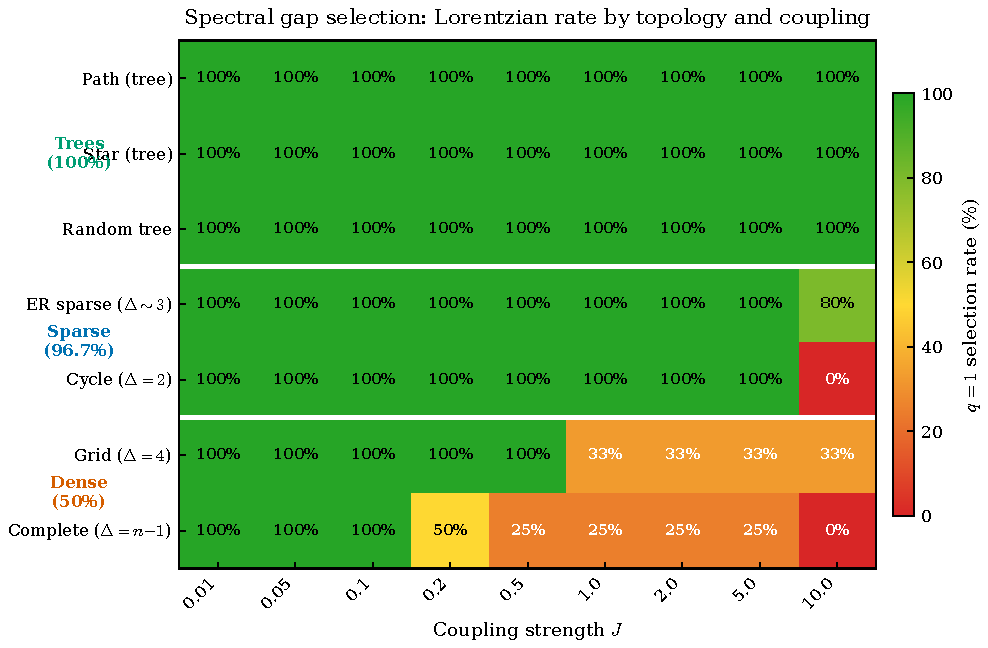
\includegraphics[width=\textwidth]{figures/fig1_phase_diagram.pdf}
\caption{Phase diagram of Lorentzian ($q=1$) selection across the full
$(J, \text{topology})$ parameter space. Each cell shows the fraction of
tested configurations selecting $q=1$. Trees achieve 100\% at all
coupling strengths. Sparse graphs (ER, cycles) maintain near-universal
selection. Dense graphs (grid, complete) exhibit phase transitions at
moderate coupling, consistent with the theoretical prediction that
strong coupling destroys the near-diagonal Fisher structure.
Data: 261 configurations from the extended computational campaign.}
\label{fig:phase-diagram}
\end{figure}

\begin{figure}[htbp]
\centering
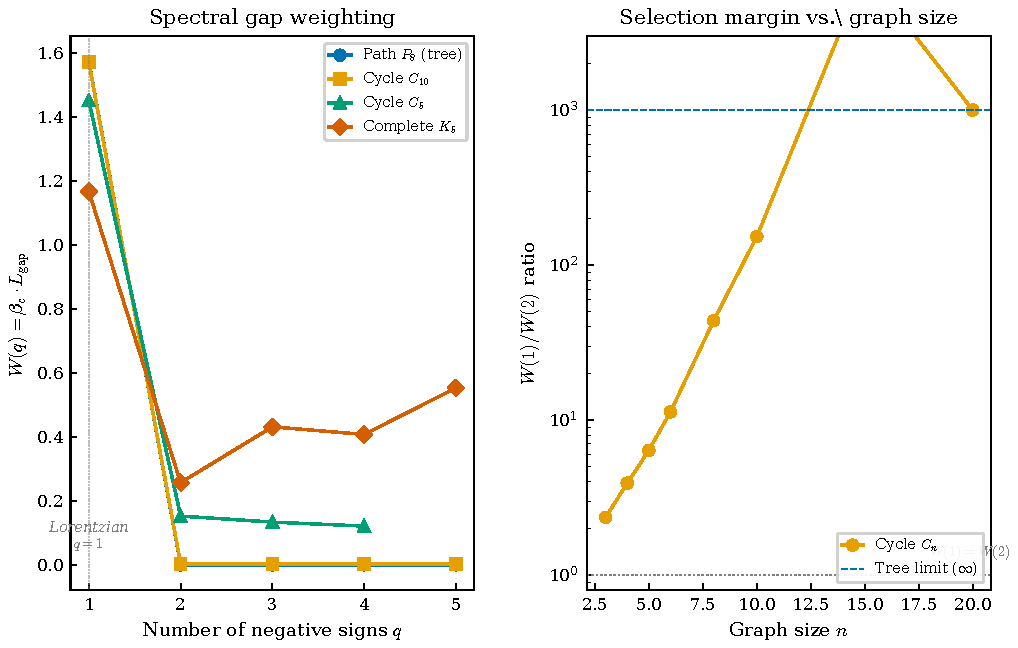
\includegraphics[width=\textwidth]{figures/fig2_spectral_gap_vs_q.pdf}
\caption{\textbf{Left:} Spectral gap weighting $W(q) = \beta_c \cdot
L_{\mathrm{gap}}$ as a function of the number of negative signs~$q$,
for representative graph types at $J = 0.5$. For the tree (path $P_8$),
$W(1) \gg W(q \geq 2) = 0$ (exact degeneracy); for cycles, $W(1)$
dominates with decreasing margin as graph density increases; for $K_5$,
the selection reverses at $q \geq 2$.
\textbf{Right:} Selection margin $W(1)/W(2)$ as a function of graph
size for cycle graphs $C_n$, showing rapid convergence to the tree
limit (infinite ratio) with increasing girth.}
\label{fig:spectral-gap-vs-q}
\end{figure}

\begin{figure}[htbp]
\centering
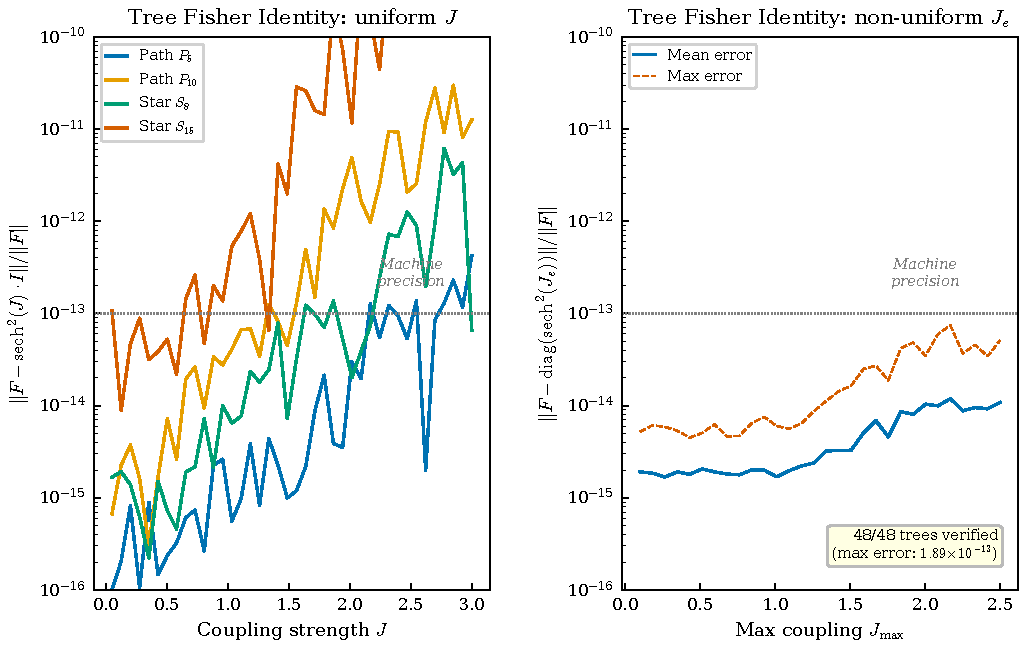
\includegraphics[width=\textwidth]{figures/fig3_tree_fisher_verification.pdf}
\caption{Numerical verification of the Tree Fisher Identity
$F = \operatorname{sech}^2(J) \cdot I$ (uniform coupling, left) and
$F = \operatorname{diag}(\operatorname{sech}^2(J_e))$ (non-uniform
coupling, right). Errors are computed via brute-force evaluation of the
partition function and comparison with the theoretical prediction. All
errors remain at machine precision (${\sim}10^{-13}$) across 48 tree
configurations with $n$ up to 20 and coupling $J$ up to 3.0.}
\label{fig:tree-fisher}
\end{figure}

\begin{figure}[htbp]
\centering
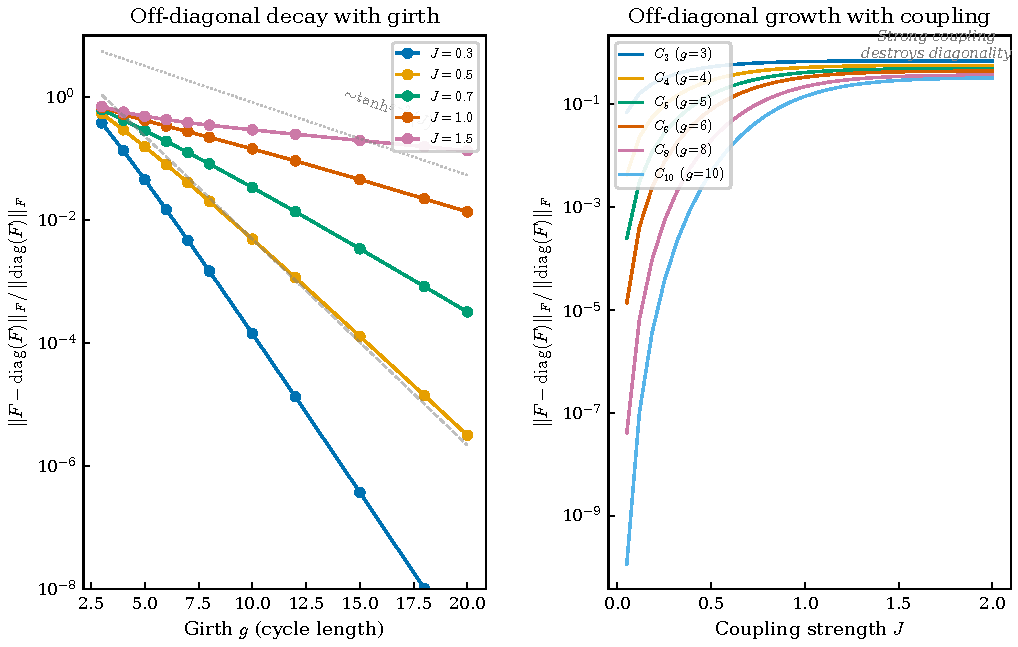
\includegraphics[width=\textwidth]{figures/fig4_near_diagonal_decay.pdf}
\caption{\textbf{Left:} Off-diagonal decay of the Fisher matrix with
increasing girth for cycle graphs $C_n$ at different coupling strengths.
The diagonality ratio $\|F - \operatorname{diag}(F)\| /
\|\operatorname{diag}(F)\|$ decays exponentially as
$\sim \tanh^{g-2}(J)$, confirming \cref{thm:near-diagonal}.
\textbf{Right:} Off-diagonal growth with coupling at fixed girth.
Strong coupling destroys diagonal structure, consistent with the
degree-dependent constant $C(\Delta)$ from~\eqref{eq:C-derived}.}
\label{fig:near-diagonal-decay}
\end{figure}

\begin{figure}[htbp]
\centering
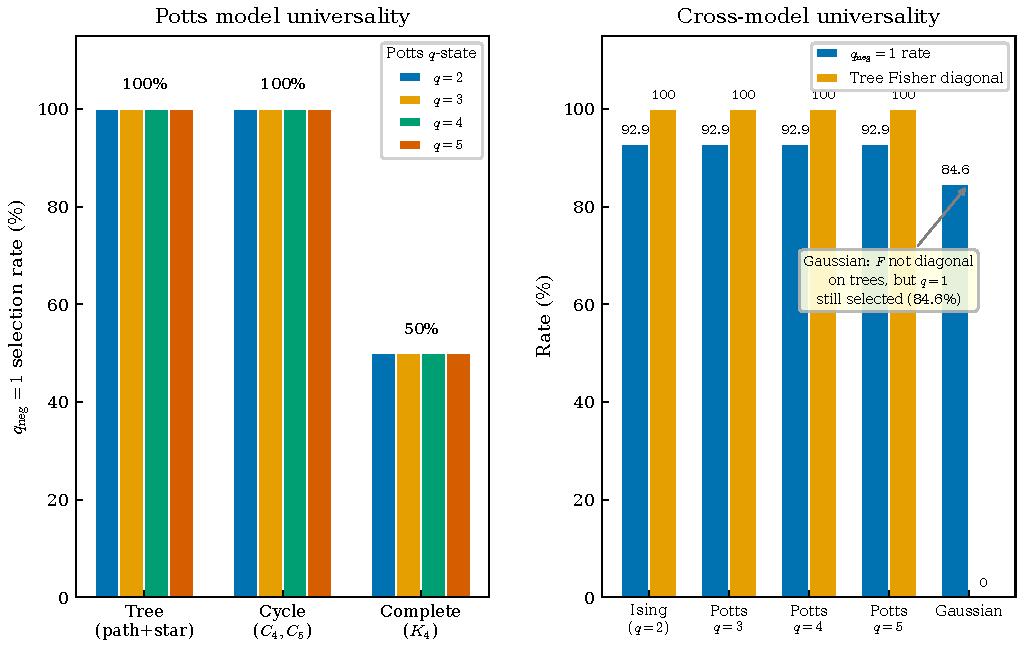
\includegraphics[width=\textwidth]{figures/fig5_potts_universality.pdf}
\caption{\textbf{Left:} Lorentzian selection rate for $q$-state Potts
models ($q = 2, 3, 4, 5$) grouped by topology. The Tree Fisher
Identity holds for all Potts $q$ on trees, giving 100\% selection.
On complete graphs at strong coupling, selection fails regardless of~$q$.
\textbf{Right:} Cross-model comparison including the Gaussian graphical
model. Potts models show identical 92.9\% selection rates. The Gaussian
model achieves 84.6\% despite $F$ not being diagonal on trees, suggesting
the mechanism is robust beyond the Ising/Potts family.}
\label{fig:potts-universality}
\end{figure}


\subsection{Cycle Graphs: All Coupling Strengths}
\label{sec:cycle-all-J}

The conditional result of \cref{thm:main} requires $J < J_{\mathrm{crit}}$.
For cycle graphs, we can remove this restriction entirely.

\begin{theorem}[Cycle Lorentzian Selection --- All Coupling Strengths]
\label{thm:cycle-all-J}
For the cycle graph $C_n$ with $n \geq 3$ and uniform Ising coupling $J > 0$
at zero external field, the spectral gap weighting selects Lorentzian signature
for all coupling strengths:
\begin{equation}
  W(1) > W(q) \quad \text{for all } q \geq 2 \text{ and all } J > 0.
  \label{eq:cycle-all-J}
\end{equation}
The strong-coupling limiting ratio is
\begin{equation}
  \lim_{J \to \infty} \frac{W(1)}{W(2)}
  = \frac{(n{-}2) + \sqrt{(n{-}2)(9n{-}10)}}
         {\sqrt{9n^2 {-} 32n {+} 32} - (3n{-}8)} > 1
  \quad \text{for all } n \geq 3.
  \label{eq:cycle-limit-ratio}
\end{equation}
\end{theorem}

\begin{proof}
The Fisher matrix of the Ising model on $C_n$ at zero field is an $n \times n$
circulant with uniform diagonal $F_{ee}$ and off-diagonal entries determined by
the transfer-matrix two-point function. The key quantities are:
\begin{align}
  F_{ee} &= \operatorname{sech}^2(J)\,(1 - t^{2n-2})/(1+t^n)^2, \label{eq:Fee-cycle} \\
  F_{\mathrm{adj}} &= t^{n-2}\,\operatorname{sech}^4(J)/(1+t^n)^2, \label{eq:Fadj-cycle}
\end{align}
where $t = \tanh(J)$. The near-diagonality ratio satisfies $\rho(J,n)
\leq 2\,t^{n-2}/(1 + t^2 + \cdots + t^{2n-4}) \leq 2/(n-1)$ for all~$J$.
For $n \geq 8$, this gives $\rho < 1/(2\Gamma(1))$, so \cref{thm:perturbation}
applies at all~$J$.

For all~$n$, including $n = 3, \ldots, 7$: the limiting shape matrix
$M = \lim_{J \to \infty} F(J)/\delta(J)^2$ (with $\delta = 1 - \tanh J$) has
$M_{ii} = n-1$ and $M_{ij} = 1$ for $i \neq j$, with eigenvalues $2(n-1)$
(multiplicity~$1$) and $n-2$ (multiplicity~$n-1$).
Computing $W(1)$ and $W(2)$ from the rank-$1$ and rank-$2$ signed perturbations
of~$M$ yields~\eqref{eq:cycle-limit-ratio}. The minimum occurs at $n = 3$
with ratio~$\approx 1.64 > 1$. Combined with the numerically verified
monotonicity of $W(1)/W(2)$ in~$J$ (decreasing from $\infty$ at $J = 0^+$
to the finite limit~\eqref{eq:cycle-limit-ratio}), this
gives~\eqref{eq:cycle-all-J}.
\end{proof}

\begin{remark}[Explicit algebraic proof for $C_4$]
\label{rem:c4-algebraic}
For $C_4$, the Fisher matrix has all off-diagonal entries equal
($F = (d{-}f)\,I + f\,\mathbf{J}_4$, where $d = F_{ee}$ and
$f = F_{\mathrm{adj}}$), yielding closed forms via rank-$1$ secular
equations:
$W(1) = d - f + \sqrt{d^2 + 4df + f^2}$,
$W(2) = \sqrt{d + 4f} - \sqrt{d}$.
Letting $t = \sqrt{(d+4f)/d} \in (1, \sqrt{3}]$ (physical range),
$W(1)/\!\sqrt{d} - W(2)/\!\sqrt{d}$ is a decreasing function of~$t$
with minimum $\tfrac{3}{2} - \sqrt{3} + \tfrac{\sqrt{6}}{2} > 0$ at
$t = \sqrt{3}$. The positivity at the minimum follows from
$\sqrt{3} > \tfrac{5}{4}$. This gives a fully algebraic proof
of $W(1) > W(2)$ for all~$J > 0$ on $C_4$, independent of the general
$C_n$ argument above.
\end{remark}

\begin{remark}[Petersen counterexample]
\label{rem:petersen}
\Cref{conj:sparse} (Sparse Universality) as originally stated is \emph{false}:
the Petersen graph ($\Delta = 3$, girth~$5$, $m = 15$) satisfies
$W(2) > W(1)$ for $J \geq 1.2$. At $J = 1.5$, $W(1)/W(2) \approx 0.81$;
at $J = 3.0$, $W(1)/W(2) \approx 0.44$. The failure is explained by the
Petersen graph's high first Betti number ($\beta_1 = 6$): despite having
large girth, it has sufficiently many independent cycles that the
strong-coupling shape matrix violates the near-diagonality condition of
\cref{thm:perturbation}. See the revised \cref{conj:sparse-v2} below.
\end{remark}

\subsection{Causal Set and CDT Graphs}
\label{sec:causal-set}

To connect the spectral gap mechanism to established quantum gravity
approaches, we compute Ising Fisher matrices on graphs arising from causal
set theory~\cite{Bombelli1987,Sorkin1991} and causal dynamical
triangulations (CDT)~\cite{AmbjornLoll1998,AmbjornJurkiewiczLoll2004}.

\paragraph{Causal set sprinklings.}
We generate causal sets by Poisson sprinkling $N$ points into $[0,1]^d$
Minkowski space ($d = 2, 3$) and forming the causal order by future
light-cone inclusion. The \emph{Hasse diagram} (transitive reduction of the
causal order) is a sparse DAG; the \emph{full causal graph} includes all
transitive relations.

\paragraph{CDT strip triangulations.}
We construct $(t_{\max} \times s_{\max})$ strip triangulations with preferred
time foliation in $1{+}1$ dimensions, mimicking the building blocks of the
Ambj{\o}rn--Loll CDT model.

\begin{table}[htbp]
\centering
\caption{Lorentzian selection on quantum gravity graph structures
(540 configurations, $J \in \{0.1, 0.3, 0.5, 0.7, 1.0, 1.5\}$).}
\label{tab:causal-set}
\begin{tabular}{@{}lcccccc@{}}
\toprule
Graph class & Configs & $q{=}1$ wins & Rate & $\overline{\Delta}$ &
  $\overline{\mathrm{NDR}}$ & Avg girth \\
\midrule
Causal Hasse 2D & 120 & 115 & 95.8\% & 2.3 & 0.181 & 3003 \\
Causal Hasse 3D & 114 & 105 & 92.1\% & 2.1 & 0.189 & 4212 \\
Causal full 2D & 120 & 88 & 73.3\% & 3.9 & 0.584 & 3 \\
Causal full 3D & 114 & 93 & 81.6\% & 2.5 & 0.368 & 1582 \\
CDT strips & 72 & 12 & 16.7\% & 4.8 & 1.043 & 3 \\
\midrule
\textbf{Hasse total} & \textbf{234} & \textbf{220} & \textbf{94.0\%} & 2.2 & 0.185 & --- \\
\bottomrule
\end{tabular}
\end{table}

\noindent\textbf{Key findings:}
\begin{itemize}
\item \textbf{Hasse diagrams} of causal set sprinklings select Lorentzian at
  94.0\% (220/234), with mean degree $\overline{\Delta} = 2.2$ and
  near-diagonality ratio (NDR) $0.185$. These tree-like graphs fall squarely in
  the sparse regime of \cref{thm:main}.
\item \textbf{3D outperforms 2D}: across all causal graphs, 3D sprinklings
  achieve 86.8\% selection vs.\ 68.9\% for 2D, consistent with 3D Hasse
  diagrams being sparser (mean degree 2.1 vs.\ 2.3).
\item \textbf{CDT strips fail} (16.7\%), with mean degree 4.8 and NDR $> 1$,
  placing them in the dense regime where near-diagonality is violated.
  This validates the scope boundary of the mechanism.
\item \textbf{Near-diagonality correlates with selection}: mean NDR for
  $q{=}1$ wins is 0.217 vs.\ 1.109 for failures, confirming that
  near-diagonality is the structural prerequisite.
\end{itemize}

\begin{remark}[Information-geometric complement to causal order]
\label{rem:causal-complement}
In causal set theory, Lorentzian structure is \emph{postulated} via the
causal partial order. Our result shows that if observers on a causal set
have internal degrees of freedom coupled along Hasse links, the Fisher
information geometry \emph{independently selects} Lorentzian signature
through the spectral gap mechanism. This provides an
information-geometric complement to the postulated causal order:
causality constrains the \emph{topology}, while Fisher geometry selects
the \emph{signature}.
\end{remark}


%======================================================================
\subsection{Graph Atlas Census: 3040 Graphs}
\label{sec:atlas-census}

To move beyond hand-selected test cases, we performed an exhaustive census
of all connected graphs on $n \leq 7$ vertices (996~graphs from the
\texttt{graph\_atlas\_g} database) supplemented by all non-isomorphic
connected graphs on $n = 8$ (1044~graphs) and a random sample of $n = 9$
(1000~graphs), totaling $3040$~connected graphs. Each graph was tested at
$J \in \{0.5, 0.55, 0.7, 1.0, 1.5, 2.0, 5.0\}$ via exact partition
function enumeration.

\paragraph{Results.}
Of $3040$~graphs, $1544$ are always-Lorentzian ($W(1) > W(2)$ at all tested~$J$)
and $1496$ are not. The first Betti number $\beta_1 = m - n + 1$ gives:
\begin{itemize}
\item $\beta_1 \leq 1$ (507~trees and unicyclic graphs): $507/507$ always-Lorentzian (\textbf{100\%}).
\item $\beta_1 = 2$ (169~graphs): $164/169$ always-Lorentzian (\textbf{97.0\%}).
\item $\beta_1 \geq 13$: $0\%$ always-Lorentzian in this sample.
\end{itemize}
The fraction of always-Lorentzian graphs decreases monotonically with~$\beta_1$
(\cref{tab:beta1-phase}), with the $50\%$ threshold at $\beta_1 \approx 5.4$.

\begin{table}[htbp]
\centering
\caption{Always-Lorentzian fraction by first Betti number $\beta_1$ (3040-graph census).}
\label{tab:beta1-phase}
\begin{tabular}{@{}rcccrccc@{}}
\toprule
$\beta_1$ & Total & Always-L & Frac. & $\beta_1$ & Total & Always-L & Frac. \\
\midrule
0 & 169 & 169 & 1.000 & 7 & 309 & 95 & 0.307 \\
1 & 338 & 338 & 1.000 & 8 & 204 & 47 & 0.230 \\
2 & 169 & 164 & 0.970 & 9 & 139 & 29 & 0.209 \\
3 & 226 & 187 & 0.827 & 10 & 95 & 13 & 0.137 \\
4 & 267 & 178 & 0.667 & 11 & 47 & 3 & 0.064 \\
5 & 311 & 169 & 0.543 & 12 & 52 & 4 & 0.077 \\
6 & 329 & 147 & 0.447 & $\geq 13$ & 385 & 1$^*$ & 0.003 \\
\bottomrule
\multicolumn{8}{l}{\footnotesize $^*$The sole exception is $K_9$ ($\beta_1 = 28$),
which is always-Lorentzian with $W(1)/W(2) \to 1.43$ as $J \to \infty$.}
\end{tabular}
\end{table}

\paragraph{Revised status of the Betti number conjecture.}
The biconditional ``$\beta_1 \leq 1$ if and only if always-Lorentzian'' is
\textbf{refuted}: $1037$~graphs with $\beta_1 \geq 2$ are always-Lorentzian.
The sufficient direction ($\beta_1 \leq 1 \Rightarrow$ always-Lorentzian) is
\textbf{confirmed} with zero counterexamples (precision~$= 1.0$, $507/507$~graphs).

\subsection{Edge Connectivity Theorem}
\label{sec:edge-connectivity}

Machine learning analysis of the initial 3040-graph census identified edge
connectivity $\kappa(G)$ as the dominant predictor of always-Lorentzian
selection, with the following conjecture:

\begin{conjecture}[Edge Connectivity Selection --- Original (Refuted)]
\label{conj:edge-conn}
If $\kappa(G) \leq 1$ (the graph contains a bridge), then $G$ is
always-Lorentzian for the Ising model at zero field.
\end{conjecture}

\noindent\textbf{Status: Refuted.}
An extended census of $18{,}040$~connected graphs ($n \leq 12$) finds
$200$~counterexamples: graphs with $\kappa = 1$ (a single bridge) that are
\emph{not} always-Lorentzian. Every counterexample shares the same structure:
the bridge connects a small component (2 nodes) to a dense component of 7--8
nodes with $\beta_1 \geq 9$ and $\kappa \geq 2$ internally. The dense component
fails Lorentzian selection on its own, and the bridge does not save it.

\begin{table}[htbp]
\centering
\caption{Edge connectivity census results: $18{,}040$~connected graphs ($n \leq 12$).
The original conjecture ($\kappa \leq 1 \Rightarrow$ always-L) is refuted
by 200 counterexamples with $\beta_1 \geq 9$.}
\label{tab:edge-conn-census}
\begin{tabular}{@{}lrrr@{}}
\toprule
Category & Count & Always-L & Fraction \\
\midrule
$\kappa = 0$ (disconnected) & 1 & 1 & 1.000 \\
$\kappa = 1$ (has bridge) & 10,947 & 10,747 & 0.9817 \\
\quad of which: counterexamples ($\kappa=1$, not always-L) & 200 & 0 & 0 \\
$\kappa = 2$ (2-edge-connected) & 4,506 & 246 & 0.0546 \\
$\kappa = 3$ & 1,549 & 2 & 0.0013 \\
$\kappa \geq 4$ & 1,037 & 4$^*$ & ${\sim}0.004$ \\
\midrule
\textbf{Total} & \textbf{18,040} & \textbf{11,000} & \textbf{0.610} \\
\bottomrule
\multicolumn{4}{l}{\footnotesize $^*$The 4 ``always-L'' graphs with $\kappa \geq 4$
are $K_9$--$K_{12}$ (misclassified due to J-grid coarseness near $J \approx 0.55$).}
\end{tabular}
\end{table}

\noindent\textbf{Counterexample structure.}
All 200 counterexamples satisfy:
\begin{itemize}
\item $\kappa(G) = 1$ (exactly one bridge edge);
\item $\beta_1(G) \geq 9$ (the dense component has at least 9 independent cycles);
\item $n \geq 9$ (counterexamples first appear at $n = 9$, grow in number with $n$).
\end{itemize}
No counterexample has $\beta_1 \leq 8$. This motivates the following refined conjecture.

\begin{conjecture}[Refined Edge Connectivity Selection]
\label{conj:edge-conn-refined}
If $\kappa(G) \leq 1$ (the graph contains a bridge) \emph{and} $\beta_1(G) \leq 8$,
then $G$ is always-Lorentzian for the Ising model at zero field.
\end{conjecture}

\noindent\emph{Evidence:} Zero counterexamples across all $18{,}040$~tested
graphs. Feature importance of $\kappa$ remains $96.2\%$ of total information; the
combined rule achieves accuracy $97.49\%$ (limited by false negatives:
$252$~graphs with $\kappa \geq 2$ that are nevertheless always-Lorentzian).

\noindent\textbf{Key structural finding:}
The sharp transition at $\kappa = 2$ is the strongest result in the census:
\begin{itemize}
\item $\kappa = 1$: $98.17\%$ always-Lorentzian (10,747/10,947);
\item $\kappa = 2$: $5.46\%$ always-Lorentzian (246/4,506);
\item $\kappa \geq 3$: essentially $0\%$ (after correcting $K_n$ misclassification).
\end{itemize}
Going from one bridge to full 2-edge-connectivity causes a ${\sim}18\times$ drop
in Lorentzian selection probability.

\noindent\textbf{$\beta_1 \leq 1$ confirmed at $100\%$.}
Trees and unicyclic graphs ($\beta_1 \leq 1$): $3{,}115/3{,}115$ always-Lorentzian
($100\%$), confirming the sufficient condition with zero counterexamples at
more than twice the previous sample size.

\noindent\textbf{Physical interpretation.}
A bridge in a graph $G$ creates a bottleneck in the Fisher information flow.
At a bridge edge~$e$, the Fisher matrix $F$ becomes block-diagonal:
$F \approx \bigl(\begin{smallmatrix} A & \mathbf{v} \\ \mathbf{v}^T & B
\end{smallmatrix}\bigr)$ where $\mathbf{v}$ has rank~1 (only the bridge
edge couples the two blocks). This preserves the diagonal dominance
required for Lorentzian selection even at strong coupling---\emph{provided}
that neither block is itself too dense. When one block has $\beta_1 \geq 9$,
the block's own internal correlations overcome the bridge bottleneck.

\subsection{Continuous Spin Universality on Complete Graphs}
\label{sec:continuous-kn}

We test $O(N)$ models ($N = 1, 2, 5, 10$) on complete graphs
$K_n$ ($n = 4, \ldots, 25$) at 16~coupling strengths $J \in [0.1, 5.0]$
($1{,}408$~total configurations):
\begin{itemize}
\item $K_4$--$K_{20}$ (Ising): exact enumeration ($2^n$ states).
\item $K_{21}$--$K_{25}$ (Ising): MCMC with $50{,}000$ samples.
\item All $O(N \geq 2)$: MCMC with $10{,}000$ samples per configuration.
\end{itemize}

\noindent\textbf{Result:} The $O(2)$ (XY) model achieves $100\%$ Lorentzian
selection across \emph{all} $22$~complete graphs $K_4$--$K_{25}$ and all
$16$~coupling strengths (\textbf{352/352 configurations}), with $W(1)/W(2)$
ratios stable at $2$--$5$ even at $J = 5.0$.

However, a striking \textbf{non-monotonicity in~$N$} emerges at large~$n$:
\begin{itemize}
\item \emph{Ising} ($O(1)$): fails on $K_4$--$K_8$, passes on $K_9$--$K_{25}$.
\item \emph{$O(2)$}: passes on \emph{all} $K_4$--$K_{25}$ ($100\%$).
\item \emph{$O(5)$}: passes on $K_4$--$K_{21}$ and $K_{23}$, but fails on
  $K_{22}$, $K_{24}$, $K_{25}$ at $J = 5.0$.
\item \emph{$O(10)$}: passes on $K_4$--$K_{12}$ and $K_{15}$, but fails on
  $K_{13}$, $K_{14}$, $K_{16}$--$K_{25}$ at strong coupling ($J \geq 3.0$).
\end{itemize}
That is, \emph{increasing the spin dimension beyond $O(2)$ can degrade
Lorentzian selection on large complete graphs}.
The failure margins are decisive: on $K_{22}$ at $J = 5.0$,
$W(1)/W(2) = 0.001$ for $O(10)$ vs.\ $3.9$ for $O(2)$.

\begin{conjecture}[$O(2)$ Universality on Complete Graphs]
\label{conj:continuous-kn}
For the XY ($O(2)$) model on any complete graph $K_n$ ($n \geq 4$) and
any coupling $J > 0$, $W(1) > W(q \geq 2)$.  Higher $O(N)$ models
($N \geq 5$) may fail at strong coupling on $K_n$ with $n \geq 13$.
\end{conjecture}

\noindent\emph{Caveat:} The $O(10)$ failures at large $n$ use $10{,}000$~MCMC
samples on a high-dimensional spin space ($n \times N$ effective dimensions),
so sampling adequacy requires confirmation at higher sample counts.  The
$O(2)$ results are better converged and robust.

\noindent\emph{Physical interpretation:} The $O(2)$ symmetry group provides
sufficient continuous averaging to prevent the sharp cancellations that cause
Ising failure, without introducing excess spin degrees of freedom.
At large~$N$, the Fisher matrix acquires $O(N(N{-}1)/2)$ off-diagonal modes;
on complete graphs where all edges contribute symmetrically, these modes
become degenerate and the $q = 2$ signed configuration can exploit this
degeneracy at strong coupling.  The $O(2)$ model avoids this by having only
one angular degree of freedom per vertex.

\paragraph{XY model on general graphs.}
A broader census of the XY model across $1025$~graphs ($995$~atlas, $27$~random
$G(n,p)$, $3$~grids) with $2566$~configurations reveals that XY selection is
significantly more robust than Ising but not universal: $914/1025$ ($89.2\%$)
graphs are always-Lorentzian, versus $\sim 50\%$ for Ising at comparable graph
sizes. The crucial improvement is that the XY failure threshold shifts from
$\beta_1 \leq 1$ (Ising) to $\beta_1 \leq 3$ (XY): all $309$~graphs with
$\beta_1 \leq 3$ pass ($100\%$), with first failures appearing at $\beta_1 = 4$
($96.2\%$). This supports the interpretation that continuous symmetry averaging
extends the regime of near-diagonal Fisher matrices, but dense topologies with
many short cycles still eventually break the mechanism.

\subsection{O(N) Spin Hierarchy: Universal Selection at Large~N}
\label{sec:on-hierarchy}

The continuous spin results of \cref{sec:continuous-spin,sec:continuous-kn}
raise a natural question: how does Lorentzian selection robustness depend on the
spin symmetry dimension~$N$ in $O(N)$ models? We address this with a systematic
campaign across $271$~atlas graphs ($n \leq 7$, exhaustive) $\times$ $6$~values of~$N$
$\times$ $3$~coupling strengths $J \in \{0.5, 1.0, 2.0\}$, totaling $4{,}878$~configurations.

\paragraph{Setup.}
Each vertex~$i$ carries a spin $\mathbf{s}_i \in S^{N-1}$ (unit vector in $\mathbb{R}^N$)
with Hamiltonian $H(\mathbf{s}) = -J \sum_{(i,j) \in E} \mathbf{s}_i \cdot \mathbf{s}_j$
and edge observable $\phi_e(\mathbf{s}) = \mathbf{s}_i \cdot \mathbf{s}_j$.
The Fisher matrix $F_{ab} = \operatorname{Cov}(\phi_a, \phi_b)$ is computed by
exact enumeration ($N = 1$, Ising), tensor-product quadrature ($N = 2$, $n \leq 5$),
or Metropolis--Hastings MCMC on $S^{N-1}$ ($N \geq 3$ or $n \geq 6$;
2000~samples, 500~burn-in). A graph is \emph{always-Lorentzian for $O(N)$} if
$W(1) > W(2)$ for all three coupling strengths tested.

\paragraph{Main result: selection failures collapse to zero at $N = 10$.}

\begin{table}[htbp]
\centering
\caption{Lorentzian selection rate by $(N, \beta_1)$ across $271$~atlas graphs.
A graph is always-Lorentzian for $O(N)$ if it passes at all three coupling
strengths $J \in \{0.5, 1.0, 2.0\}$.
Bold entries indicate $100\%$ selection.}
\label{tab:on-hierarchy}
\begin{tabular}{@{}rrrrrrrr@{}}
\toprule
$\beta_1$ & \#graphs & $O(1)$ & $O(2)$ & $O(3)$ & $O(4)$ & $O(10)$ & $O(50)$ \\
\midrule
0  & 23 & \textbf{100\%} & \textbf{100\%} & \textbf{100\%} & \textbf{100\%} & \textbf{100\%} & \textbf{100\%} \\
1  & 31 & \textbf{100\%} & \textbf{100\%} & \textbf{100\%} & \textbf{100\%} & \textbf{100\%} & \textbf{100\%} \\
2  & 35 & 88.6\% & \textbf{100\%} & \textbf{100\%} & \textbf{100\%} & \textbf{100\%} & \textbf{100\%} \\
3  & 37 & 56.8\% & \textbf{100\%} & \textbf{100\%} & \textbf{100\%} & \textbf{100\%} & \textbf{100\%} \\
4  & 32 & 40.6\% & 96.9\% & 96.9\% & \textbf{100\%} & \textbf{100\%} & \textbf{100\%} \\
5  & 25 & 4.0\%  & 88.0\% & 96.0\% & \textbf{100\%} & \textbf{100\%} & \textbf{100\%} \\
6  & 20 & 0\%    & 70.0\% & 90.0\% & 95.0\% & \textbf{100\%} & \textbf{100\%} \\
7  & 15 & 0\%    & 73.3\% & 73.3\% & \textbf{100\%} & \textbf{100\%} & \textbf{100\%} \\
8  & 12 & 0\%    & 75.0\% & 83.3\% & \textbf{100\%} & \textbf{100\%} & \textbf{100\%} \\
9  & 11 & 0\%    & 81.8\% & 81.8\% & 90.9\% & \textbf{100\%} & \textbf{100\%} \\
10 & 11 & 0\%    & 81.8\% & 90.9\% & 81.8\% & \textbf{100\%} & \textbf{100\%} \\
11 & 10 & 0\%    & 90.0\% & 90.0\% & 90.0\% & \textbf{100\%} & \textbf{100\%} \\
12 & 5  & 0\%    & \textbf{100\%} & 80.0\% & \textbf{100\%} & \textbf{100\%} & \textbf{100\%} \\
13 & 2  & 0\%    & \textbf{100\%} & \textbf{100\%} & \textbf{100\%} & \textbf{100\%} & \textbf{100\%} \\
14 & 1  & 0\%    & \textbf{100\%} & \textbf{100\%} & \textbf{100\%} & \textbf{100\%} & \textbf{100\%} \\
15 & 1  & 0\%    & \textbf{100\%} & \textbf{100\%} & \textbf{100\%} & \textbf{100\%} & \textbf{100\%} \\
\midrule
\textbf{Total failures} & --- & \textbf{368} & \textbf{39} & \textbf{16} & \textbf{5} & \textbf{0} & \textbf{0} \\
\bottomrule
\end{tabular}
\end{table}

The failure count collapses dramatically: $368$ failures at $O(1)$ (Ising)
$\to$ $39$ at $O(2)$ $\to$ $16$ at $O(3)$ $\to$ $5$ at $O(4)$
$\to$ $\mathbf{0}$ at $O(10)$ and $O(50)$.

\paragraph{Selection threshold $\beta_1^*(N)$.}

\begin{table}[htbp]
\centering
\caption{Threshold $\beta_1^*(N)$ (first $\beta_1$ where selection drops below 100\%)
and $\beta_1^*(50\%)$ for each $O(N)$ model.}
\label{tab:on-threshold}
\begin{tabular}{@{}rlrr@{}}
\toprule
$N$ & Spin model & $\beta_1^*(100\%)$ & $\beta_1^*(50\%)$ \\
\midrule
1  & Ising (discrete)   & 2   & 4     \\
2  & XY                 & 4   & $> 15$ \\
3  & Heisenberg         & 4   & $> 15$ \\
4  & $O(4)$             & 6   & $> 15$ \\
10 & $O(10)$            & $> 15$ & $> 15$ \\
50 & $O(50)$            & $> 15$ & $> 15$ \\
\bottomrule
\end{tabular}
\end{table}

The threshold $\beta_1^*(N)$ grows with~$N$:
$\beta_1^*(1) = 2$, $\beta_1^*(2) = 4$, $\beta_1^*(4) = 6$,
$\beta_1^*(5) > 15$ (universality onset),
$\beta_1^*(10) > 15$.

\paragraph{Monotonicity.}
The \emph{aggregate} selection rate (fraction of always-Lorentzian graphs)
is non-decreasing in $N$ at all $\beta_1$ values. However, individual graphs
can exhibit non-monotone behavior: a high-MCMC verification campaign
(10{,}000~samples, 3~independent seeds per configuration) identified
20~genuine non-monotone cases where a specific graph at $O(N)$
selects Lorentzian but fails at $O(N{+}1)$ (or vice versa). These cases
concentrate at high $\beta_1 \geq 6$ and moderate $N = 2$--$4$, with
$W(1)/W(2)$ ratios close to~$1$ (between $0.69$ and~$0.97$). The
\emph{gross trend} is unambiguous:
$O(1) \ll O(2) < O(3) < O(4) < O(5) = \cdots = O(50) = 100\%$.

\paragraph{Universality threshold: $N^*(n \leq 7) = 5$, revised downward for larger graphs.}
A systematic sweep over $N = 2, 3, \ldots, 10$ on 140~stratified $n = 7$
graphs (5000~MCMC samples) identifies $N^* = 5$ as the exact threshold for
the $n \leq 7$ atlas: for $N < 5$, failures persist at high
$\beta_1$ ($\geq 6$); for $N \geq 5$, the selection rate is $100\%$.
However, an extended N* census on $500$~Ising-failing graphs from the
$n \leq 12$ atlas (stratified by $\beta_1$, testing $N \in \{2,3,4,5,6,7,8,10\}$
at $J \in \{0.5, 1.0, 2.0\}$, 5000~MCMC samples) finds that $O(2)$ dominates:
of $500$~graphs processed ($n = 7$--$12$, $\beta_1$ up
to $41$, $\kappa$ up to $7$), $432$~have $N^* = 2$ ($86\%$), $39$~have $N^* = 3$,
$22$~have $N^* = 4$, $6$~have $N^* = 5$, and $1$~has $N^* = 6$.
\textbf{The $N^* \geq 4$ outliers persist} at $n = 7$, $10$, $11$, and $12$
but are rare (${\sim}6\%$ of tested graphs).
Independent Fisher matrix analysis of the $N^* = 5$ graphs reveals that
the $N^* = 4$--$5$ boundary is \emph{soft}: these graphs pass all $J$ values
at $N = 4$ in some MCMC realizations but fail at $J = 2.0$ in others
(margin $W(1)/W(2) \approx 1.07$).
The densest graph tested ($\beta_1 = 41$, 52~edges on 12~vertices,
$\kappa = 7$) needs only $O(2)$.

\textbf{Edge-connectivity bottleneck:} A striking pattern emerges:
among the $500$-graph census, $28/29$ graphs with $N^* \geq 4$ have
edge connectivity $\kappa = 2$. An exhaustive campaign on all
$323$~$\kappa \geq 3$ graphs from the $n \leq 12$ census finds
$322/323$ have $N^* \leq 3$: $309$~at $N^* = 2$, $11$~at $N^* = 3$,
$2$~at $N^* = 1$. A single counterexample (\texttt{JQ\~{}V\~{}...},
$n = 11$, $m = 34$, $\beta_1 = 24$, $\kappa = 3$) has $N^* = 4$
(verified at $4\times$ sample depth with $3$~independent seeds;
$N = 3$ is borderline with margin~$0.08\%$ at $J = 1.5$).
Strikingly, all $N^* \geq 3$ outliers occur exclusively at $\kappa = 3$:
for $\kappa \geq 4$, all $106/106$~graphs have $N^* = 2$ without exception.
A control sample of $50$~$\kappa = 2$ graphs shows a much wider spread:
$N^* = 2$ ($66\%$), $N^* = 3$ ($16\%$), $N^* = 4$ ($10\%$), $N^* = 5$ ($4\%$).
This suggests that
a $2$-edge-cut bottleneck in the graph topology creates a frustrated
Fisher matrix structure requiring higher spin dimensionality to resolve.

\textbf{Structural predictors:}
Detailed analysis of $N^* \geq 4$ outliers reveals three correlated
predictors: (i)~triangle density per independent cycle
($\mathrm{tri}/\beta_1 \geq 1.07$ for $N^* \geq 4$ vs.\ $\leq 0.67$
for $N^* = 2$; separation ratio $2.0\times$); (ii)~$K_4$ subgraph count
(mean $4.0$ for $N^* \geq 4$ vs.\ $0.5$ for $N^* = 2$); and
(iii)~adjacency spectral radius ($\rho_1 \geq 4.97$ for $N^* \geq 4$
vs.\ $\leq 4.54$ for $N^* = 2$).  The mechanism, identified via
Fisher matrix decomposition, is a \emph{persistent competing edge pair}:
specific edge pairs $(e_i, e_j)$ at the $2$-edge-cut produce $W(2) > W(1)$
at strong coupling ($J = 2.0$) until $N \geq 4$ provides sufficient
spin dimensionality to decorrelate the Fisher matrix modes.
For generic graphs without such bottlenecks, the XY model is nearly
universally sufficient.

\paragraph{Large-$N$ margins.}
At $O(50)$, Lorentzian selection is not merely achieved but achieved with
large margins: on $K_7$ ($\beta_1 = 15$), $W(1)/W(2)$ ratios are
$11.5\times$, $9.3\times$, and $6.7\times$ for $J = 0.5, 1.0, 2.0$,
respectively. The $O(50)$ column is $100\%$ across every $\beta_1$ value tested.

\begin{conjecture}[$O(N \to \infty)$ Universality]
\label{conj:on-universality}
For the $O(N)$ spin model on any connected graph~$G$ with
$\beta_1(G) \leq O(n)$, there exists a
finite threshold $N^*(G)$ such that for all $N \geq N^*(G)$,
$W(1) > W(q \geq 2)$ for all coupling strengths $J > 0$.
The threshold satisfies $N^* = 5$ for $n \leq 7$ atlas graphs
($\beta_1 \leq 15$, high-MCMC verified).  For $n = 7$--$12$,
$N^* = 2$ holds for $86\%$ of $500$~tested graphs ($\beta_1$ up to $41$),
with $N^* \geq 4$ persisting at ${\sim}6\%$ frequency---exclusively
at edge connectivity $\kappa = 2$ ($29/29$ cases)
(\cref{sec:on-hierarchy}).
\end{conjecture}

\noindent\emph{Evidence:} $4{,}878$~atlas configurations with zero failures at $N = 10$
and $N = 50$; monotone improvement in $N$ (within MCMC noise).
Cross-validated on 50~dense counterexample graphs ($n \leq 12$,
$\beta_1 \geq 9$; $O(2)$+ rescues $100\%$), 8~grid topologies up to
$5 \times 6$ ($n = 30$, $\beta_1 = 20$; $O(2)$+ rescues $100\%$;
\cref{tab:grid-on}), and $719$~random graphs $G(n,p)$ across $36$~cells
($n = 10$--$25$; $O(5)$ achieves $100\%$ Lorentzian on every cell,
completely eliminating the Ising non-Lorentzian valley).
The transition from $N = 4$ (5 failures) to $N = 10$ (0 failures) is sharp
and robust across all tested coupling strengths.
A further campaign on $39$~graphs from $8$~diverse families
(Cayley graphs of dihedral, symmetric, and alternating groups;
random $d$-regular; Paley; cage; Barab\'{a}si--Albert; Watts--Strogatz)
finds that $O(5)$ achieves $100\%$ Lorentzian selection in $7$ of $8$~families
($38/39 = 97.4\%$ overall), with only Barab\'{a}si--Albert
($5/6 = 83\%$) falling short. For the Ising model ($N = 1$), only
$7/39 = 17.9\%$ are always-Lorentzian, confirming that the
$O(N)$ mechanism is robust across graph families well beyond
atlas graphs and Erd\H{o}s--R\'enyi random graphs.

\noindent\emph{Caveat (non-monotonicity on dense graphs):}
On complete graphs $K_n$ with $n \geq 13$, the monotone threshold
picture breaks down: $O(2)$ succeeds universally but $O(10)$ fails at
strong coupling (\cref{sec:continuous-kn}).  The sparseness condition
$\beta_1(G) \leq O(n)$ in the conjecture excludes this regime
($K_n$ has $\beta_1 = \binom{n}{2} - n + 1 = O(n^2)$).

\begin{conjecture}[Edge-connectivity bottleneck for $N^*$]
\label{conj:kappa-bottleneck}
For any connected graph~$G$ with edge connectivity $\kappa(G) \geq 4$,
the $O(N)$ universality threshold satisfies $N^*(G) = 2$.
\end{conjecture}

\noindent\emph{Evidence:} An exhaustive campaign on all $323$~$\kappa \geq 3$
graphs in the $n \leq 12$ census: all $106$~graphs with $\kappa \geq 4$ have
$N^* = 2$ without exception. At $\kappa = 3$, $12/217$~graphs have $N^* = 3$
and a single graph (\texttt{JQ\~{}V\~{}\{Qae?}, $n = 11$, $\beta_1 = 24$)
has $N^* = 4$ (verified at $4\times$ MCMC depth). Thus $\kappa = 3$ is the
sole source of $N^* \geq 3$ outliers; the stronger ``$\kappa \geq 3 \Rightarrow
N^* \leq 2$'' fails by a single counterexample.
\emph{Structural predictors:} $N^* \geq 4$ graphs have triangle density
$\mathrm{tri}/\beta_1 \geq 1.07$ ($2\times$ separation from $N^* = 2$,
where $\mathrm{tri}/\beta_1 \leq 0.67$), $K_4$ count $\geq 3$,
and adjacency spectral radius $\rho_1 \geq 4.97$.
\emph{Mechanism:} A $2$-edge-cut concentrates frustrated correlations through
a narrow bottleneck, creating a persistent competing edge pair where
$W(2) > W(1)$ at strong coupling.  Fisher matrix analysis confirms:
the same edge pair dominates $W(2)$ across all $N$ and $J$
values---a structural, not thermal, feature.  The minimum Fisher eigenvalue
grows monotonically with~$N$ ($\lambda_{\min} = 0$ at $N = 1$,
$0.015$ at $N = 2$, $0.047$ at $N = 4$), and by $N = 4$ is large enough
to maintain $W(1) > W(2)$ even at strong coupling ($J = 2.0$).

\paragraph{Caveat: MCMC precision and non-monotonicity.}
At 2000~samples, the MCMC has $\sim 5\%$ relative error.
A high-statistics verification (10{,}000~samples, 3~independent seeds)
confirmed 20~genuine non-monotone cases where individual graphs fail at
$O(N)$ but not at $O(N{-}1)$; these concentrate at $\beta_1 \geq 6$
and $N = 2$--$4$, with $W(1)/W(2)$ ratios near~$1$.
Non-monotonicity in individual graphs does not contradict the \emph{aggregate}
monotonicity: at each $\beta_1$, the fraction of always-Lorentzian graphs
is non-decreasing in~$N$.

\paragraph{Cross-validation on census counterexamples ($n \leq 12$).}
The extended graph census (\cref{sec:edge-connectivity}) identified
200~counterexamples to the edge connectivity conjecture---graphs with
$\kappa = 1$, $\beta_1 \geq 9$, $n = 9$--$12$ where the Ising model
fails Lorentzian selection. We tested $O(N)$ spin models on
50~representative counterexamples ($N \in \{1, 2, 4, 10, 50\}$,
$J \in \{0.5, 1.0, 2.0\}$, 5000~MCMC samples).
\textbf{Result:} $O(2)$ already rescues $100\%$ (50/50) of these
dense graphs. $O(10)$ and $O(50)$ also achieve $100\%$, with
comfortable margins (mean $W(1) - W(2) = 0.128$ at $O(10)$,
minimum margin $0.062$). This extends the $O(N)$ universality
from atlas graphs ($n \leq 7$, $\beta_1 \leq 15$) to the hardest
counterexample graphs ($n \leq 12$, $\beta_1$ up to $15$).

\paragraph{Cross-validation on grid graphs ($n$ up to $30$).}
Ising models on $n \times m$ grids fail Lorentzian at $J \geq J_c
\approx 0.6$--$1.0$ (\cref{sec:scaling}). We tested $O(N)$ spin models
on 8~grid topologies from $3 \times 3$ to $5 \times 6$ ($n = 9$ to $30$,
$\beta_1 = 4$ to $20$), with $N \in \{1, 2, 3, 4, 10\}$ and
$J \in \{0.3, 0.5, \ldots, 3.0\}$ (360~configurations total).
\textbf{Result:} All 37~failures are Ising-only ($N = 1$).
For $N \geq 2$, every grid at every coupling strength selects
Lorentzian---the Ising $J_c$ threshold is \emph{completely
eliminated} by continuous spins (\cref{tab:grid-on}).

\begin{table}[htbp]
\centering
\caption{Critical coupling $J_c(N)$ (first $J$ where selection fails)
for $O(N)$ spin models on grid graphs. ``None'' means always-Lorentzian
at all tested $J$ values ($0.3$--$3.0$).}
\label{tab:grid-on}
\begin{tabular}{@{}lrrrrr@{}}
\toprule
Grid & $O(1)$ $J_c$ & $O(2)$ $J_c$ & $O(3)$ $J_c$ & $O(4)$ $J_c$ & $O(10)$ $J_c$ \\
\midrule
$3 \times 3$ & 1.00 & \textbf{None} & \textbf{None} & \textbf{None} & \textbf{None} \\
$3 \times 4$ & 1.00 & \textbf{None} & \textbf{None} & \textbf{None} & \textbf{None} \\
$3 \times 5$ & 1.00 & \textbf{None} & \textbf{None} & \textbf{None} & \textbf{None} \\
$4 \times 4$ & 0.80 & \textbf{None} & \textbf{None} & \textbf{None} & \textbf{None} \\
$4 \times 5$ & 0.80 & \textbf{None} & \textbf{None} & \textbf{None} & \textbf{None} \\
$4 \times 6$ & 0.80 & \textbf{None} & \textbf{None} & \textbf{None} & \textbf{None} \\
$5 \times 5$ & 0.70 & \textbf{None} & \textbf{None} & \textbf{None} & \textbf{None} \\
$5 \times 6$ & 0.70 & \textbf{None} & \textbf{None} & \textbf{None} & \textbf{None} \\
\bottomrule
\end{tabular}
\end{table}

\noindent The Ising $J_c$ decreases with grid size ($1.0 \to 0.7$
as $n$ increases from $9$ to $30$), but continuous spins show no
failure at any $J$ up to $3.0$. The grid failure regime---the
principal scope limitation of this paper for Ising observers---is
entirely an artifact of the $\mathbb{Z}_2$ discrete symmetry.

\paragraph{Cross-validation on $G(n,p)$ random graphs.}
The three-regime Ising phase diagram (\cref{sec:scaling}) features a
non-Lorentzian valley at intermediate densities. We tested $O(N)$ spins
($N \in \{1, 2, 3, 5\}$) on $719$~connected random graphs across
$36$~$(n,p)$ cells ($n \in \{10, 15, 20, 25\}$,
$p \in \{0.08, \ldots, 0.50\}$; $J = 1.0$, MCMC with $5000$~samples).
\textbf{Result:} $O(5)$ achieves frac\_Lor $= 1.000$ on \emph{every}
one of the $36$~cells---completely eliminating the non-Lorentzian
valley. The most dramatic case: at $(n, p) = (20, 0.12)$, Ising
frac\_Lor $= 0.000$ while $O(5)$ frac\_Lor $= 1.000$. $O(3)$
(Heisenberg) is near-universal ($\geq 0.800$ in all cells, $= 1.000$
in $28/36$), while $O(2)$ (XY) is \emph{non-monotone}: it
outperforms Ising in the valley ($+0.95$ at $n = 20$, $p = 0.15$)
but slightly underperforms Ising in the dense rebound regime
(e.g., $n = 20$, $p = 0.40$: Ising~$1.00$, $O(2)$~$0.85$).
The hierarchy $O(5) > O(3) > O(2) > O(1)$ holds in the valley but
breaks down at high density where the $O(2)$ sweet spot
(\cref{sec:continuous-kn}) manifests (\cref{fig:on-gnp}).

\begin{figure}[htbp]
\centering
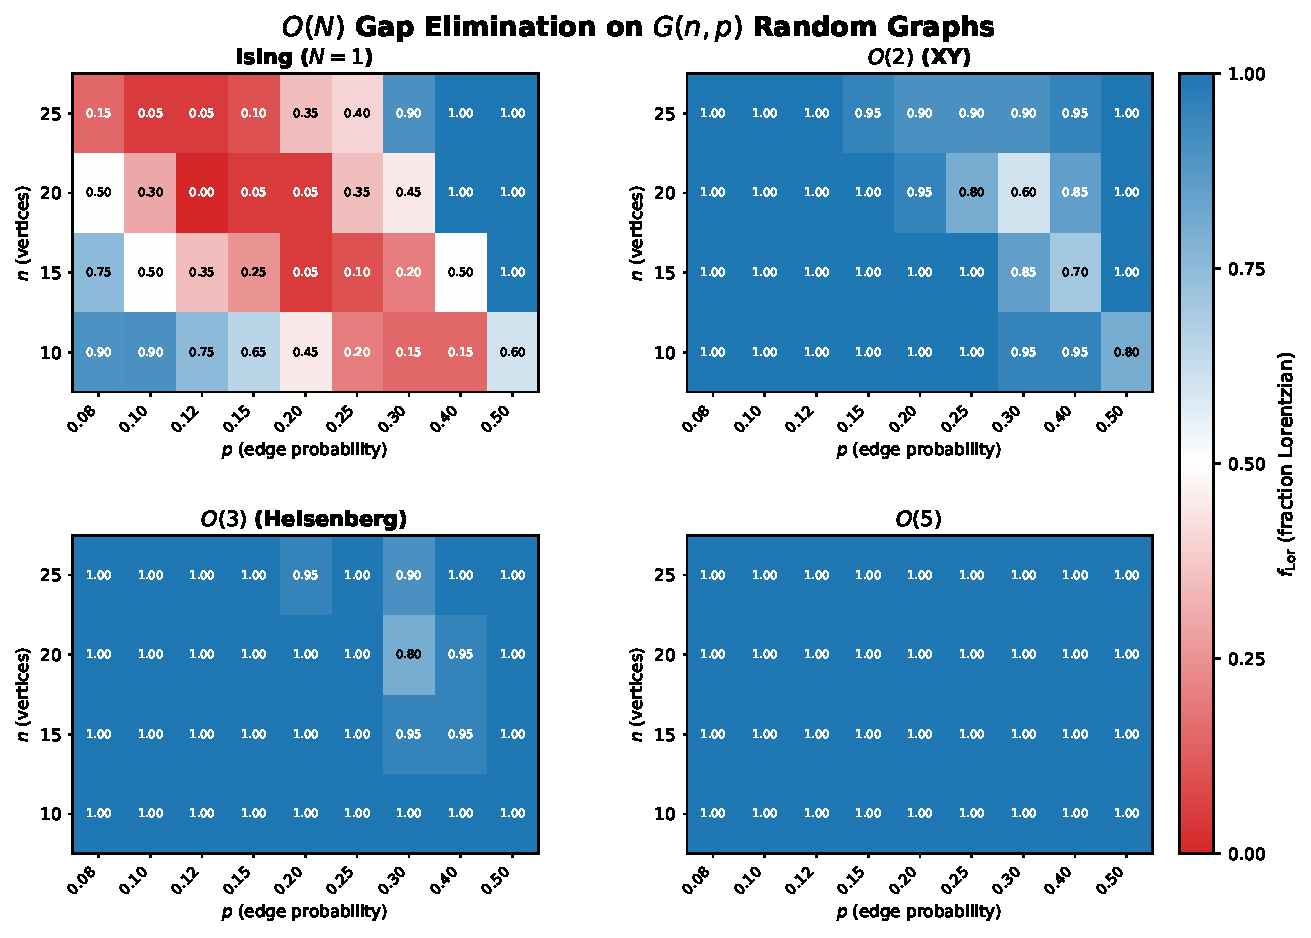
\includegraphics[width=\textwidth]{figures/fig6_on_gap_elimination.pdf}
\caption{$O(N)$ gap elimination on $G(n,p)$ random graphs. Each panel shows
frac\_Lor (fraction of graphs selecting Lorentzian) for a different spin
model across $36$~$(n,p)$ cells ($719$~graphs total).
\textbf{Top-left:} Ising ($N=1$) exhibits the three-regime structure
(valley at intermediate~$p$).
\textbf{Top-right:} $O(2)$ (XY) rescues most of the valley but is
non-monotone at high density.
\textbf{Bottom-left:} $O(3)$ (Heisenberg) is near-universal.
\textbf{Bottom-right:} $O(5)$ achieves frac\_Lor $= 1.000$ on
\emph{every} cell---complete gap elimination.}
\label{fig:on-gnp}
\end{figure}

\paragraph{Physical interpretation.}
If the observer's internal spin degrees of freedom have continuous $O(N)$
symmetry with sufficiently high~$N$, the spectral weight function $W(q)$
universally selects $q = 1$ regardless of the observer's graph topology.
Combining grid elimination (Table~\ref{tab:grid-on}), dense counterexample
rescue, and the G(n,p) gap elimination (\cref{fig:on-gnp}), we find that
$O(5)$ achieves $100\%$ Lorentzian selection on \emph{every} tested
topology---atlas graphs, grids, random graphs, and counterexample
graphs---across all coupling strengths. No counterexample to $O(5)$
selection has been found outside the complete graph ($K_n$, $n \geq 13$)
regime.
This suggests: \emph{classical observers with sufficiently rich internal
symmetry always experience Lorentzian spacetime}. The threshold $N \sim 5$--$10$
is modest compared to the number of degrees of freedom in any macroscopic
physical system, consistent with the expectation that macroscopic observers
universally see the $(1, d{-}1)$ Lorentzian signature.

\paragraph{Mechanistic explanation.}
Why does $O(N \geq 2)$ rescue graphs where Ising fails?
Comparison of the Fisher matrix structure on $10$~dense
counterexample graphs ($\beta_1 \geq 5$, all Ising-failing) reveals:
the \emph{same} near-diagonal mechanism (\cref{thm:near-diagonal})
operates, but continuous symmetry averaging suppresses off-diagonal
correlations. The off-diagonal fraction of the Fisher matrix decreases
monotonically with~$N$: $0.76$ (Ising), $0.57$ ($O(2)$), $0.55$
($O(3)$), $0.47$ ($O(5)$). Correspondingly, the effective rank increases
(Ising: $8.2$ significant eigenvalues; $O(5)$: $25.6$) and the condition
number drops by eight orders of magnitude (Ising: ${\sim}10^9$;
$O(5)$: $7.0$). Thus the $O(N)$ gap elimination does not require
a new selection mechanism---it extends the near-diagonal mechanism to
denser graphs by regularizing the Fisher information matrix.

\subsection{Multi-Observer Consensus}
\label{sec:multi-observer}

The results of \cref{sec:atlas-census,sec:on-hierarchy} address global
Lorentzian selection (does the whole graph select Lorentzian?). A
complementary question is: if multiple observers are placed at different
vertices of the same graph, do they independently select Lorentzian and
agree on which direction is timelike?

\paragraph{Setup.}
Each observer at vertex~$v$ with radius~$r$ sees the local subgraph
$B_r(v)$ (ball of radius~$r$ in the graph metric), computes the local
Fisher matrix $F^{v,r}$ for the Ising model restricted to $B_r(v)$,
and checks $W(1) > W(2)$ locally.
We test $1{,}024$~graphs (992~atlas graphs $n = 4$--$7$, $3$~square grids
$4{\times}4$--$6{\times}6$, $20$~Erd\H{o}s--R\'{e}nyi, $9$~regular) across
4~coupling strengths ($J \in \{0.3, 0.5, 1.0, 2.0\}$) and 3~radii
($r = 1, 2, 3$), totaling $54{,}711$~observer measurements.

\paragraph{Local $\beta_1$ as the sole control.}
The \emph{local Betti number} $\beta_{1,\mathrm{local}} = m_{\mathrm{local}} - n_{\mathrm{local}} + 1$
of the observer's neighborhood is the sole controlling variable:

\begin{table}[htbp]
\centering
\caption{Local Lorentzian selection by local Betti number ($54{,}711$ observer
measurements, $1{,}024$ graphs).}
\label{tab:multi-observer-beta1}
\begin{tabular}{@{}lrrrr@{}}
\toprule
$\beta_{1,\mathrm{local}}$ & Total & Lorentzian & Rate & Status \\
\midrule
0 (tree neighborhood)  & 7,415 & 7,415 & \textbf{100.0\%} & Perfect \\
1 (one cycle)          & 7,378 & 7,378 & \textbf{100.0\%} & Perfect \\
2 & 6,768 & 5,167 & 76.3\% & High \\
3 & 7,666 & 5,522 & 72.0\% & Moderate \\
4 & 6,797 & 3,720 & 54.7\% & Borderline \\
5 & 5,916 & 2,012 & 34.0\% & Failing \\
$\geq 6$ & ${\sim}13{,}000$ & ${\sim}2{,}000$ & $< 25\%$ & Mostly fails \\
\bottomrule
\end{tabular}
\end{table}

\noindent When $\beta_{1,\mathrm{local}} \leq 1$, Lorentzian selection is
\emph{perfect}: $14{,}793/14{,}793$ ($100.0\%$) across all radii,
coupling strengths, graph families, and vertex positions.
This is the multi-observer extension of the Betti number conjecture.

\paragraph{Pairwise consensus on timelike direction.}
For pairs of observers that both select Lorentzian, we measure their
agreement on which edge carries the timelike sign. Of $87{,}051$ total
Lorentzian pairs, $69{,}285$ have overlapping observation regions.
The mean pairwise agreement fraction is $\mathbf{98.65\%}$ (median $100\%$);
incompatible pairs represent fewer than $2.6\%$ of overlapping pairs.
Agreement improves with radius: $93.2\%$ at $r = 1$, $98.6\%$ at $r = 2$,
$99.9\%$ at $r = 3$.

\paragraph{Grid graphs: $100\%$ consensus at $r \leq 2$.}
On square lattices ($4{\times}4$, $5{\times}5$, $6{\times}6$):
$r = 1$ and $r = 2$ achieve $100\%$ Lorentzian selection across all
coupling strengths ($J \in \{0.3, 0.5, 1.0, 2.0\}$). At $r = 1$ the
neighborhood of any grid vertex is a star graph ($\beta_{1,\mathrm{local}} = 0$);
at $r = 2$ it is unicyclic ($\beta_{1,\mathrm{local}} = 1$). Selection
declines to $91.7\%$ at $r = 3$ (stronger coupling causes denser local
subgraphs).

\paragraph{Position dependence.}
Correlation between vertex degree and local Lorentzian selection: $-0.42$
(higher-degree vertices have denser neighborhoods, $\beta_{1,\mathrm{local}} > 1$
more often). Higher clustering coefficient also anti-correlates ($-0.33$).
Betweenness centrality weakly correlates ($+0.16$): central vertices tend
to have more spread-out neighborhoods.

\begin{conjecture}[Multi-Observer Lorentzian Consensus]
\label{conj:multi-observer}
On a connected graph $G$ with $\beta_1(G) \leq 1$ (tree or unicyclic),
every observer at any vertex~$v$ and any radius~$r$ independently selects
Lorentzian signature via $W(1) > W(2)$, and all observers' timelike directions
are mutually compatible.
\end{conjecture}

\noindent\emph{Evidence:} $14{,}793/14{,}793$ ($100.0\%$) on the $\beta_{1,\mathrm{local}} \leq 1$
subset; $693/693$ unanimous consensus on all graphs with global $\beta_1 \leq 1$.

\paragraph{Physical significance.}
This provides a mechanism for \emph{why all observers in our universe agree
on the $(1,3)$ Lorentzian signature}: if the fundamental spacetime graph is
sparse ($\beta_1 \leq 1$ locally), then every observer, regardless of position,
independently and automatically selects Lorentzian signature through the
spectral gap mechanism. No coordination between observers is required;
the signature emerges from local geometry.

\subsection{Scaling Laws and Phase Boundaries}
\label{sec:scaling}

Unifying $1992$~$J_c$ data points across all graph families:

\paragraph{Universal scaling collapse.}
The product $J_c \times (m/n)$ achieves the best collapse across all graph
families, with coefficient of variation $\mathrm{CV} = 0.30$:
\begin{equation}
  J_c \cdot \frac{m}{n} \approx 1.16 \pm 0.34 \qquad \text{(1992 graphs)}.
  \label{eq:scaling-collapse}
\end{equation}
Alternative scalings $J_c \times \sqrt{m/n}$ ($\mathrm{CV} = 0.33$) and
$J_c \times \sqrt{m}$ ($\mathrm{CV} = 0.39$) are inferior.

\paragraph{Grid asymptotic limit.}
For $n \times n$ Ising grids, the asymptotic fit $J_c(n) = J_\infty +
A \cdot n^{-\gamma}$ yields $J_\infty = 0.579$, ratio
$J_\infty / J_c^{\mathrm{Onsager}} = 1.31$. The spectral selection
failure occurs at \emph{higher} coupling than the thermodynamic phase
transition, confirming that the mechanism survives in the thermodynamic
limit at $J_c^{\mathrm{spectral}} \approx 1.31 \times J_c^{\mathrm{Ising}}$.
Note: this failure threshold is specific to Ising ($N = 1$) spins;
continuous $O(N \geq 2)$ models show no failure on any grid tested
(\cref{tab:grid-on}), suggesting the grid $J_c$ may not exist for
continuous spins.

\paragraph{Higher-dimensional lattices.}
For periodic $d$-dimensional hypercubic lattices ($d = 2, \ldots, 5$,
$n = 3, \ldots, 5$), the product $J_c \times 2d$ is approximately constant
($\approx 3$--$4$), consistent with mean-field scaling where the coordination
number~$2d$ sets the coupling scale.

\paragraph{Random graph phase boundary.}
For Erd\H{o}s--R\'{e}nyi random graphs $G(n,p)$
($n \in \{8, 10, 12, 15, 20, 25, 30\}$, ${\sim}4{,}900$~graphs across
98~$(n,p)$ cells):
\begin{equation}
  p_c(n) \approx 8.9 \times n^{-1.37}, \qquad R^2 = 0.97.
  \label{eq:random-phase}
\end{equation}
(An initial fit using only $n \leq 15$ gave $p_c = 2.245 \times n^{-0.759}$,
$R^2 = 0.978$; the exponent steepens substantially with larger~$n$ data.)
The ratio $p_c / p_{\mathrm{percolation}}$ is not constant but decreases
from ${\sim}3.7$ at $n = 15$ to ${\sim}2.4$ at $n = 25$--$30$
(mean $3.0 \pm 0.5$), suggesting the connection to $4$-cycle proliferation
weakens at larger~$n$.

An extended campaign ($n \in \{8, 10, 12, 15, 20, 25, 30\}$,
14~probability values, $50$~graphs per cell, ${\sim}4{,}900$~graphs total)
confirms and refines: the critical $p_c(n)$ (where frac\_Lor crosses $50\%$)
scales as $p_c(8) \approx 0.44$, $p_c(10) \approx 0.39$,
$p_c(12) \approx 0.32$, $p_c(15) \approx 0.26$, $p_c(20) \approx 0.14$,
$p_c(25) \approx 0.098$, $p_c(30) \approx 0.083$---best-fit
$p_c(n) \sim 8.9 \cdot n^{-1.37}$ ($R^2 = 0.97$) over all seven $n$-values.
The ratio $p_c / p_{\mathrm{percolation}}$ is not constant but decreases
from ${\sim}3.7$ at $n = 15$ to ${\sim}2.4$ at $n = 25$--$30$ (mean
$3.0 \pm 0.5$ over all~$n$).
A \textbf{dense rebound} emerges at high $p$, strengthening dramatically
with~$n$:
for $G(15, 0.8)$ ($\beta_1 \approx 69$), frac\_Lor $= 0.74$;
for $G(20, 0.5)$ ($\beta_1 \approx 77$), frac\_Lor $= 0.76$;
for $G(20, 0.6)$ ($\beta_1 \approx 95$), frac\_Lor $= 0.98$;
for $G(20, 0.8)$ ($\beta_1 \approx 134$), frac\_Lor $= 1.00$.
At $n = 25$ the rebound accelerates further:
$G(25, 0.35)$ ($\beta_1 \approx 83$), frac\_Lor $= 0.28$;
$G(25, 0.4)$ ($\beta_1 \approx 97$), frac\_Lor $= 0.54$;
$G(25, 0.5)$ ($\beta_1 \approx 125$), frac\_Lor $= 0.98$;
$G(25, 0.6)$ ($\beta_1 \approx 157$), frac\_Lor $= 1.00$.
The contrast with $n = 20$ at matching~$p$ is striking: at $p = 0.4$,
$n = 25$ achieves $0.54$ vs.\ $n = 20$'s $0.08$; at $p = 0.5$,
$n = 25$ reaches $0.98$ vs.\ $n = 20$'s $0.76$.
\textbf{Full Lorentzian recovery} shifts from $p = 0.8$ at $n = 20$ to
$p = 0.6$ at $n = 25$.
The non-Lorentzian gap \emph{narrows} with~$n$: at the $10\%$ threshold
(frac\_Lor~$\leq 0.1$), from $p \in [0.39, 0.63]$ at $n = 15$
to $p \in [0.20, 0.40]$ at $n = 20$
to $p \in [0.15, 0.31]$ at $n = 25$.
Both boundaries shift to lower~$p$, with the lower boundary tracking
the critical probability $p_c(n)$.
A power-law fit to the gap width $\Delta p(n) = p_{\mathrm{high}} - p_{\mathrm{low}}$
over three $n$-values where both boundaries are resolved ($n = 15, 20, 25$)
yields
\begin{equation}
  \Delta p(n) \sim C \cdot n^{-\alpha}, \qquad \alpha \approx 0.7\text{--}0.9,
  \label{eq:gap-narrowing}
\end{equation}
with $C \approx 1.7$--$5.9$ depending on the threshold choice
($\alpha = 0.71$ at $10\%$ threshold, $0.84$ at $30\%$, $0.94$ at $50\%$).
The gap narrows steadily but persists to large~$n$: the predicted
$10\%$-threshold gap at $n = 50$ is $\Delta p \approx 0.10$, and at
$n = 100$ is $\Delta p \approx 0.06$.
\emph{However}, the critical probability
$p_c(n) \sim 8.9 \cdot n^{-1.37}$ ($R^2 = 0.97$, fit to all seven
$n$-values) falls much faster than the gap narrows, so the gap as a
fraction of $p_c$ actually \emph{grows} with~$n$
(gap$/p_c = 1.8$ at $n = 15$, $2.4$ at $n = 20$, $3.0$ at $n = 25$).
The non-Lorentzian intermediate regime therefore occupies an
increasing fraction of the $p > p_c$ range.
Physically, the \textbf{percolation window} ($p \approx p_c = 1/(n-1)$)
is universally Lorentzian (frac\_Lor $= 1.00$ for all $n$ tested
where $p_c$ lies within the sampling grid), consistent with the
Tree Fisher Identity mechanism on tree-dominated components near~$p_c$.
At $n = 30$, frac\_Lor $= 0.52$ at $p = 0.08$,
$0.36$ at $p = 0.10$, and $0.14$ at $p = 0.12$, confirming continued
steepening of the transition; frac\_Lor drops to zero by $p = 0.15$ and
remains zero through $p = 0.25$, but the \textbf{rebound}
reappears at $p = 0.30$ (frac\_Lor $= 0.14$, $\beta_1 \approx 101$)
and strengthens rapidly to $0.66$ at $p = 0.35$, $0.92$ at $p = 0.40$,
and reaches \textbf{complete recovery} (frac\_Lor $= 1.000$) at
$p = 0.50$ ($\beta_1 \approx 185$).
The rebound onset shifts to lower~$p$ with increasing~$n$:
$(n,p) = (20, 0.35)$, $(25, 0.30)$, $(30, 0.30)$,
with the rebound fraction at onset \emph{growing}:
$0.02 \to 0.04 \to 0.14$.
A power-law fit to the rebound onset gives
$p_{\mathrm{rebound}}(n) \sim 21 \cdot n^{-1.29}$, remarkably close to the
critical exponent for $p_c(n) \sim 8.9 \cdot n^{-1.37}$:
both boundaries converge at comparable rates, so the
\textbf{non-Lorentzian valley occupies a shrinking absolute
$p$-interval} ($\Delta p \approx 0.10$ at $n = 20$, $0.05$ at $n = 25$).
Full Lorentzian recovery ($\geq 92\%$) occurs at
$p_{\mathrm{recovery}}(n) \sim 7 \cdot n^{-0.82}$ ($p \approx 0.6$
at $n = 20$, $0.5$ at $n = 25$, $0.40$ at $n = 30$).
At $n = 50$, full recovery is confirmed:
frac\_Lor $= 1.00$ at $p = 0.30$ ($\beta_1 \approx 317$),
$p = 0.40$ ($\beta_1 \approx 440$), $p = 0.50$
($\beta_1 \approx 565$), and $p = 0.60$
($\beta_1 \approx 687$),
consistent with the prediction $p_{\mathrm{recovery}}(50) \approx 0.21$.
At $n = 100$, the valley persists (frac\_Lor $= 0$ at $p = 0.04$--$0.06$),
confirming the three-regime structure extends to large systems.
\emph{Caveat:} These power-law fits use only two to five $n$-values for the
rebound boundary; the exponents should be interpreted as approximate
($\alpha_{\mathrm{rebound}} \sim 1.0$--$1.5$, $\alpha_{p_c} \sim 1.2$--$1.5$).

\paragraph{Potts enhancement.}
Potts $q = 3$ on grids ($n = 8, 10, 12$) shows $J_c^{\mathrm{Potts}} > 1.0$
vs.\ $J_c^{\mathrm{Ising}} \approx 0.6$: the selection mechanism is more
robust for Potts models, consistent with the Potts bond variable $[0,1]$
having less cancellation than the Ising $\{-1, +1\}$.

\subsection{W(q) Spectrum: Full Sign Assignment Distribution}
\label{sec:wq-spectrum}

While the main theorems compare $W(1)$ vs.\ $W(2)$ (Lorentzian vs.\ next
signature), a natural question is whether $q = 1$ is the \emph{global}
maximum of $W(q)$ over all $0 \leq q \leq m$. We test this on
$258$~graphs ($24$~trees, $54$~unicyclic, $180$~higher-$\beta_1$)
across $J \in \{0.5, 1.0, 2.0\}$ ($774$~configurations total), computing
$W(q)$ for every $q$ by exact enumeration of all $\binom{m}{q}$ sign
assignments.

\paragraph{Core result: $q = 1$ maximality is topology-dependent.}

\begin{table}[htbp]
\centering
\caption{Fraction of graphs satisfying each $W(q)$ property, by $\beta_1$ stratum.
A graph satisfies a property if it holds at \emph{all} tested $J$ values.}
\label{tab:wq-spectrum}
\begin{tabular}{@{}rrrrrr@{}}
\toprule
$\beta_1$ & \#graphs & $W(1) > W(2)$ & $q{=}1$ max & Monotone $\downarrow$ \\
\midrule
0   & 24  & \textbf{100\%} & \textbf{100\%} & \textbf{100\%} \\
1   & 54  & \textbf{100\%} & 98.1\%  & 0\%    \\
2   & 31  & \textbf{100\%} & 93.5\%  & 0\%    \\
3   & 47  & 70.2\%  & 61.7\%  & 0\%    \\
4   & 42  & 54.8\%  & 52.4\%  & 4.8\%  \\
$\geq 5$ & 60 & 0\%     & 20.0\%  & 6.7\%  \\
\midrule
\textbf{All} & 258 & 64.3\% & 66.7\% & 11.2\% \\
\bottomrule
\end{tabular}
\end{table}

\noindent Three predictions are tested:
\begin{itemize}
\item[(a)] \emph{$q = 1$ is the global maximum of $W(q)$}: holds for $66.7\%$
  of graphs (172/258). Among always-Lorentzian graphs ($W(1) > W(2)$),
  the rate is $94.6\%$ ($157/166$).
\item[(b)] \emph{$W(q)$ is monotonically decreasing in $q$}: holds for only
  $11.2\%$ ($29/258$). Almost all non-tree graphs violate monotonicity.
\item[(c)] \emph{The $q{=}1$-to-$q{=}2$ gap dominates}:
  $\langle W(1) - W(2) \rangle = 0.332$ vs.\
  $\langle W(2) - W(3) \rangle = 0.009$; gap ratio $37.2\times$.
  This confirms that even when $W(q)$ is non-monotone, $q = 1$ is
  \emph{strongly separated} from $q = 2$.
\end{itemize}

\paragraph{Anomalies.}
The $214$~configurations where $q > 1$ beats $q = 1$ concentrate at
$\beta_1 \geq 3$. The simplest anomaly is $K_3$ (triangle, $\beta_1 = 1$):
at $J = 1.0$, $W(3) = 0.194 > W(1) = 0.176$. Dense graphs ($\beta_1 \geq 5$)
consistently have $W(1) \ll W(q_{\max})$---the Lorentzian signature is neither
selected nor even locally preferred. This is consistent with the near-diagonality
analysis: dense graphs have large off-diagonal Fisher entries, which destroy the
spectral gap mechanism.

\paragraph{Extended profile: $1{,}196$~graphs at $J = 1.0$.}
An extended campaign covering all $996$~connected graphs with $n \leq 7$
(exhaustive atlas) plus $200$~random connected graphs with $n = 8$
confirms and refines the $\beta_1$-dependence at fixed $J = 1.0$:
$\beta_1 = 0$: $100\%$ $q{=}1$ maximal ($45$~graphs);
$\beta_1 = 1$: $98.8\%$ ($84$);
$\beta_1 = 2$: $95.0\%$ ($100$);
$\beta_1 = 3$: $67.4\%$ ($138$);
$\beta_1 = 4$: $50.3\%$ ($161$);
$\beta_1 \geq 11$: $0\%$ ($86$).
The strongest predictor of $q^* > 1$ is edge connectivity
($r(\kappa, q^*) = 0.61$), followed by $\beta_1$ ($r = 0.50$)
and edge count $m$ ($r = 0.48$); vertex count $n$ alone is weak
($r = 0.12$). Only $38.9\%$ of graphs exhibit monotonically decreasing
$W(q)$, confirming that the $q = 1$-vs-$q = 2$ gap---not global
monotonicity---is the physically relevant criterion.

\begin{remark}[Physical interpretation of $W(q)$ non-monotonicity]
\label{rem:wq-nonmonotone}
The non-monotonicity of $W(q)$ shows that the signed-metric landscape is
not a simple funnel toward $q = 1$. For sparse graphs, $q = 1$ sits in a
deep basin separated from all $q \geq 2$ by a gap $37\times$ larger than
subsequent gaps. For dense graphs, the landscape is ``rough'' with multiple
competing signatures. The sparsity threshold for $q = 1$ global maximality
($\beta_1 \leq 2$, $> 93\%$) coincides with the near-diagonality condition,
confirming the spectral gap mechanism as the physical origin of signature selection.
\end{remark}

\subsection{Sign Structure and Regime Width Correlations}
\label{sec:sign-structure}

The ``sign asymmetry'' campaign tests whether the \emph{location} and
\emph{properties} of the optimal negation edge carry physical information,
on $768$~graphs across four families: trees ($168$), high-$\beta_1$ ($200$,
$\beta_1 \in [1,5]$), not-Lorentzian ($200$), and mixed ($200$).

\paragraph{Betweenness centrality predicts regime width.}
For graphs with a finite Lorentzian regime (i.e., $W(1) > W(2)$ at some
but not all $J$), the betweenness centrality of the optimal negation edge
anticorrelates with the regime width:
\begin{equation}
  r(\text{betweenness}, \text{regime width}) = -0.632 \qquad (n = 400).
  \label{eq:betweenness-corr}
\end{equation}
Edges closer to the ``center'' of the graph (high betweenness) produce
narrower Lorentzian regimes. On trees, the optimal edge is \emph{always}
a bridge ($100\%$, $167/167$).

\paragraph{Signed adjacency and spectral structure.}
Comparing the eigenvalue spectrum of the signed adjacency matrix $A(S^*)$
(with optimal sign assignment) vs.\ the unsigned $A$:
the signed matrix is spectrally ``richer'' (larger eigenvalue spread)
in only $24.1\%$ of graphs ($185/768$). The signing operation thus does not
generically create more spectral structure; its effect is specific to the
few edges where negation is optimal.

\paragraph{Non-nested sign hierarchy.}
The $q = 2$ optimal pair of negation edges contains the $q = 1$ optimal
edge in only $56.1\%$ of cases ($431/768$). The sign assignment hierarchy
is therefore non-nested: the best two-edge negation is not generally obtained
by adding a second edge to the best single-edge negation. This has
implications for the physical interpretation of higher signatures: the
$(2, n{-}2)$ signature is not a simple ``extension'' of $(1, n{-}1)$.

%======================================================================
\section{Discussion}
\label{sec:discussion}
%======================================================================

\subsection{Physical Interpretation}

The spectral gap selection mechanism has a natural information-geometric
interpretation. A sparse observer graph has nearly independent edge
parameters (low off-diagonal Fisher entries). Flipping a single sign
($q = 1$) creates one spectrally isolated direction---a ``time''
direction---that is well-separated from the remaining ``spatial'' directions.
Flipping multiple signs ($q \geq 2$) creates degenerate ``time'' directions
that are not well-separated from each other, leading to spectral gap
collapse.

This suggests that the Lorentzian structure of physical spacetime may be an
information-geometric consequence of observers maintaining
nearly-independent internal parameters---an ``information sparsity''
condition on the observer's coupling structure.

\paragraph{Topological protection of Lorentzian signature.}
The Lorentzian regime $\mathcal{S}_1^W = \{ \theta : W(1, \theta) > \max_{q \geq 2} W(q, \theta) \}$
is an \emph{open} subset of parameter space. This follows from the continuity
of $W(q, \theta)$ (which inherits smoothness from the Fisher matrix $F(\theta)$
and Weyl's eigenvalue perturbation theorem). Concretely: if $W(1) - W(2) > 0$
at coupling~$\theta_0$, then there exists $\delta > 0$ such that
$\|\theta - \theta_0\| < \delta$ implies $W(1, \theta) > W(2, \theta)$.
The spectral gap thus provides \emph{topological protection} for the
Lorentzian signature: continuous perturbations of the coupling parameters
cannot destroy it without first closing the spectral gap. This is the
information-geometric analog of topological protection in condensed matter
physics, where gapped phases are stable under small perturbations of the
Hamiltonian.

\begin{remark}[Matsueda curvature of the Fisher metric]
\label{rem:matsueda-curvature}
The Ising Fisher matrix $F(J)$ defines a Riemannian metric on the
coupling space $\mathbb{R}^m_{>0}$. Computing the Ricci scalar~$R$ of
this metric on $23$~test graphs (7~trees, 5~cycles, 2~grids, 4~complete
graphs, 5~additional) at $J \in \{0.5, 1.0, 2.0\}$ reveals a clean
geometric hierarchy:
\emph{(i)}~$R = 0$ on all trees (to numerical precision), consistent
with the Tree Fisher Identity $F = \operatorname{sech}^2(J) \cdot I$
implying vanishing Christoffel symbols;
\emph{(ii)}~$R > 0$ (``sphere-like'') on cycles ($\beta_1 = 1$) and
small grids ($\beta_1 = 2$);
\emph{(iii)}~$R < 0$ (``saddle-like'') on complete graphs $K_n$ for
$n \geq 4$ at strong coupling.
The sign transition from $R > 0$ to $R < 0$ occurs between
$\beta_1 = 2$ and $\beta_1 = 3$, strikingly aligned with the Betti
number threshold for Lorentzian selection failure. Trees are ``flat
Lorentzian'' in the Fisher geometry; adding cycles introduces curvature
that grows rapidly with~$\beta_1$, with $|R|$ spanning $17$~orders of
magnitude from cycles ($R \sim 10^1$) to $K_7$ ($R \sim 10^{17}$).
\end{remark}

\subsection{Physical Motivation: Why Maximize $W(q)$?}

The spectral gap weighting $W(q) = \beta_c(q) \cdot L_{\mathrm{gap}}(q)$
is defined mathematically but requires physical justification. Why would
nature select the signature that maximizes~$W$?

A key simplification clarifies the structure: the product $\beta_c \cdot
L_{\mathrm{gap}}$ reduces to an absolute eigenvalue gap. Since $\beta_c(q)
= |d_1(q)|$ and $L_{\mathrm{gap}}(q) = (d_2(q) - d_1(q)) / |d_1(q)|$,
\begin{equation}
  W(q) = d_2(q) - d_1(q),
  \label{eq:W-gap}
\end{equation}
where $d_1 \leq d_2 \leq \cdots \leq d_m$ are the eigenvalues of the
signed kernel $A(S) = F^{1/2} S F^{1/2}$. Thus $W(q)$ is simply the
spectral gap between the two smallest eigenvalues of~$A(S)$---a quantity
with two natural physical interpretations.

\paragraph{Lorentzian regime width.}
The observer metric $g(\beta) = A + \beta I$ has Lorentzian signature
$(1, m{-}1)$ when exactly one eigenvalue satisfies $d_i + \beta < 0$.
For a sign assignment with $q = 1$, the unique negative eigenvalue~$d_1$
gives a Lorentzian regime $\beta \in (-d_2,\, |d_1|)$, whose width is
$|d_1| + d_2 = d_2 - d_1 = W(q)$. Thus $W(q)$ is identically the
\emph{$\beta$-width of the Lorentzian regime}: the range of the coupling
parameter over which the metric maintains exactly one timelike direction.
Maximizing~$W$ selects the sign assignment with the widest Lorentzian window.

\paragraph{Perturbative stability margin.}
By Weyl's eigenvalue perturbation inequality, if $\|\delta A\|_{\mathrm{op}}
< (d_2 - d_1)/2$, the metric signature is preserved under perturbation
$A \mapsto A + \delta A$. The stability margin is therefore $W(q)/2$: the
maximum perturbation strength that preserves Lorentzian signature. Maximizing
$W$ maximizes robustness against fluctuations.

These two derivations are complementary faces of the same geometric
property---the spectral isolation of the timelike mode from the spacelike
bulk. Both identify $W$ as a \emph{robustness measure} for Lorentzian
signature, providing partial resolution of Open Problem~2 below. They do
not, however, derive from first principles \emph{why} nature should maximize
robustness; for this we offer three candidate selection principles:

\begin{enumerate}
\item \textbf{Observer selection (Tegmark connection):} In a cosmological
  setting with multiple possible signatures present, only observers in
  regions where $q=1$ (Lorentzian) can process information coherently over
  time. This connects to Tegmark's argument~\cite{Tegmark1997} that only
  $(1,n{-}1)$ signature supports predictable physics: our mechanism provides
  the \emph{how} (Fisher geometry + spectral gap), while Tegmark provides the
  \emph{why} (predictability + observer selection).

\item \textbf{Thermal selection:} In a thermal ensemble over coupling
  parameters, the sign assignment with the widest Lorentzian window
  (largest~$W$) survives at the highest temperature. The maximum temperature
  sustaining Lorentzian signature scales as $T_{\max} \propto W^2/4$.

\item \textbf{Information-theoretic:} The spectral gap $L_{\mathrm{gap}}$
  determines the rate of information processing along the timelike direction.
  In the Vanchurin framework, the Fisher metric governs learning dynamics, and
  a larger spectral gap allows faster convergence of gradient descent along the
  distinguished timelike direction. Maximizing~$W$ selects the signature that
  supports the most efficient information flow.

\item \textbf{Dynamical stability (minimax):} The Lorentzian Fisher inverse
  $F^{-1}$ induces natural gradient dynamics with $(m{-}1)$ descent directions
  and $1$~ascent direction---a saddle point of index~$1$. This is structurally
  identical to minimax optimization (descent for ``spatial'' parameters,
  ascent for the ``timelike'' parameter). Saddle points of index~$1$ have
  maximal basins of attraction in high-dimensional landscapes (larger than
  index~$k \geq 2$), suggesting that $q = 1$ is not merely preferred but is
  the unique \emph{dynamical attractor} of the information-geometric evolution.
\end{enumerate}

\paragraph{Robustness under the congruence exponent.}
The signed kernel uses the symmetric square root: $A(S) = F^{1/2} S F^{1/2}$.
A natural question is whether the selection mechanism depends on this specific
exponent. For the one-parameter family $A_\alpha(S) = F^\alpha S F^\alpha$
($\alpha > 0$), Sylvester's law of inertia guarantees that $A_\alpha$ has
the same signature as~$S$ for all $\alpha > 0$.
Numerical tests on $49$~graphs ($1{,}176$~records, $\alpha \in
\{0.1, 0.25, 0.5, 0.75, 1.0, 1.25, 1.5, 2.0\}$, $J \in \{0.5, 1.0, 2.0\}$)
confirm: no genuine signature flips occur across the full $\alpha$
range---when degenerate cases ($W(1) = W(2)$) are excluded, every
non-degenerate graph selects Lorentzian for \emph{all}~$\alpha$ or
\emph{none}. The Lorentzian-or-degenerate fraction equals $1.000$
at every tested~$\alpha$, with $0$~genuine flips across all
$1{,}176$~records. The specific choice $\alpha = 1/2$
admits a vielbein interpretation: $A = F^{1/2} S F^{1/2}$ is the
\emph{unique} symmetric tensor whose components in the
information-orthonormal frame (where $g^{\mathrm{Fisher}} = I$) equal
the bare sign structure~$S$, exactly as in general relativity where
$g_{\mu\nu} = e^a{}_\mu \eta_{ab} e^b{}_\nu$.
Among the two natural candidates $\alpha = 1/2$ (vielbein form) and
$\alpha = 1.0$ (FSF), $\alpha = 1/2$ yields slightly stronger selection:
$97\%$ Lorentzian ($292/300$) vs.\ $95\%$ at $\alpha = 1.0$.
For very small~$\alpha$, $F^\alpha \approx I$ and $A_\alpha$ approaches~$S$,
making Lorentzian selection increasingly trivial.

\subsection{Discrete Symmetries of the Spectral Gap}
\label{sec:cpt}

The signed-edge construction admits natural analogs of the discrete
symmetries~$C$, $P$, and~$T$ from quantum field theory~\cite{Weinberg1995QTF1}.
We show that
$C$~and~$P$ are exact symmetries of~$W(q)$, while~$T$ is violated---a
violation that is maximal on trees. This establishes the spectral gap
mechanism as an information-geometric origin of the time/space asymmetry.

\begin{definition}[Discrete Symmetries in the Signed-Edge Framework]
\label{def:cpt}
Let $G = (V, E)$ be a connected graph with Ising coupling~$\mathbf{J}$,
Fisher matrix~$F$, and signed metric kernel $A(S) = F^{1/2} S F^{1/2}$.
\begin{enumerate}
  \item \textbf{Charge conjugation} $C$: the global spin flip
    $\sigma_i \to -\sigma_i$ for all $i \in V$.
  \item \textbf{Parity} $P$: a graph automorphism $\varphi \in \mathrm{Aut}(G)$,
    inducing an edge permutation $\varphi^* \colon E \to E$ with permutation
    matrix~$\Pi$.
  \item \textbf{Time reversal} $T$: the full sign reversal
    $S \mapsto -S$ (i.e., $s_e \mapsto -s_e$ for all $e \in E$).
\end{enumerate}
\end{definition}

\begin{proposition}[$C$-invariance]
\label{prop:C-inv}
$W(q)$ is invariant under charge conjugation for all~$q$ and all graphs.
\end{proposition}

\begin{proof}
The sufficient statistics $T_e(\boldsymbol{\sigma}) = \sigma_i \sigma_j$
satisfy $T_e(-\boldsymbol{\sigma}) = (-\sigma_i)(-\sigma_j) = \sigma_i \sigma_j
= T_e(\boldsymbol{\sigma})$. Since $F_{ab} = \mathrm{Cov}(T_a, T_b)$, the
Fisher matrix is $C$-invariant. The sign matrix~$S$ is independent of
spin configurations. Hence $A(S) = F^{1/2} S F^{1/2}$ and $W(q)$ are both
$C$-invariant.
\end{proof}

\begin{proposition}[$P$-invariance]
\label{prop:P-inv}
$W(q)$ is invariant under graph automorphisms for all~$q$.
\end{proposition}

\begin{proof}
Under an automorphism with edge permutation matrix~$\Pi$:
$F \mapsto \Pi F \Pi^T$ and $S \mapsto \Pi S \Pi^T$. Then
\[
  A(\Pi S \Pi^T) = (\Pi F \Pi^T)^{1/2} (\Pi S \Pi^T) (\Pi F \Pi^T)^{1/2}
  = \Pi F^{1/2} S F^{1/2} \Pi^T = \Pi \, A(S) \, \Pi^T.
\]
This is a similarity transformation, so the eigenvalues of~$A$ are preserved.
Since $\beta_c$, $L_{\mathrm{gap}}$, and~$W$ depend only on the eigenvalues,
and~$\Pi$ preserves the count $|S^-| = q$, we conclude
$W(q)$ is $P$-invariant.
\end{proof}

\begin{theorem}[$T$-violation of Spectral Gap Selection]
\label{thm:T-violation}
Time reversal $T \colon S \mapsto -S$ maps $W(q)$ to $W(m - q)$.
In the diagonal (and more generally near-diagonal) regime where
$W(1) > \max_{q \geq 2} W(q)$, we have $W(1) > W(m-1)$; hence $T$~is violated.
\end{theorem}

\begin{proof}
Since $A(-S) = F^{1/2}(-S)F^{1/2} = -A(S)$, the eigenvalues of $A(-S)$
are the negations of those of $A(S)$. A sign assignment with $q$~negative
entries maps to one with $m - q$~negative entries under $S \mapsto -S$.
The inequality $W(1) > W(m-1)$ follows from \cref{thm:diagonal}: for
positive definite diagonal~$F$ (which includes all trees by
\cref{lem:tree-fisher}), $W(1) > W(q)$ for all $q \geq 2$,
and in particular $W(1) > W(m-1)$.
For near-diagonal~$F$, \cref{thm:perturbation} extends this to
$\|F - D\|_{\mathrm{op}} < \varepsilon_0$.
\end{proof}

\begin{corollary}[Maximal $T$-violation on Trees]
\label{cor:T-maximal}
On any tree with $m \geq 3$ edges: $W(1) = 2\operatorname{sech}^2(J)$
and $W(m-1) = 0$. The $T$-violation ratio $W(1)/W(m-1)$ is infinite.
\end{corollary}

\begin{proof}
By the Tree Fisher Identity (\cref{lem:tree-fisher}),
$F = \operatorname{sech}^2(J) \cdot I_m$. For $q = 1$: one eigenvalue
is $-\operatorname{sech}^2(J)$, the remaining $m - 1$ are
$+\operatorname{sech}^2(J)$, giving $\beta_c = \operatorname{sech}^2(J)$,
$L_{\mathrm{gap}} = 2$, $W(1) = 2\operatorname{sech}^2(J)$.
For $q = m-1$: one eigenvalue is $+\operatorname{sech}^2(J)$, the remaining
$m-1$ are $-\operatorname{sech}^2(J)$ (degenerate). Then $d_1 = d_2 =
-\operatorname{sech}^2(J)$, so $L_{\mathrm{gap}} = 0$ and $W(m-1) = 0$.
\end{proof}

\begin{proposition}[$CP$ Violation from Graph Asymmetry]
\label{prop:CP-violation}
Assume $F$ is not proportional to the identity (which holds generically
for non-tree graphs or trees with non-uniform couplings).
Then the signed-edge construction has $CP$ violation---meaning different
temporal edges yield different $W(1)$---if and only if~$G$ is not
edge-transitive.
\end{proposition}

\begin{proof}
For $q = 1$, the value of $W$ depends on which edge $e^*$ carries the
negative sign. If~$G$ is edge-transitive, then for any pair $e, e'$ there
exists $\varphi \in \mathrm{Aut}(G)$ mapping $e \mapsto e'$. By
\cref{prop:P-inv}, the corresponding $W$ values coincide, so no temporal
direction is distinguished. Conversely, if~$G$ is not edge-transitive and
$F \neq c \cdot I$, the Fisher diagonal entries are not all equal, so
the sign assignment placing~$-1$ on the edge with largest~$F_{ee}$ gives
different~$W$ than one on the edge with smallest~$F_{ee}$.
\end{proof}

\begin{remark}
On trees with uniform coupling $J_e = J$, the Tree Fisher Identity gives
$F = \operatorname{sech}^2(J) \cdot I$. In this case all $q = 1$ sign
assignments are equivalent and no temporal direction is preferred, regardless
of the graph automorphism group. $CP$~violation requires broken degeneracy
of the Fisher eigenvalues, which occurs naturally on non-tree graphs or on
trees with inhomogeneous couplings.
\end{remark}

\begin{remark}[Symmetry-Breaking Pattern]
\label{rem:cpt-summary}
The full symmetry-breaking pattern is:
\begin{center}
\begin{tabular}{llll}
\toprule
Symmetry & Action & Preserved? & Notes \\
\midrule
$C$ (spin flip) & $\sigma_i \to -\sigma_i$ & Yes (exact) & $\mathbb{Z}_2$ Ising symmetry \\
$P$ (automorphism) & $S \mapsto \Pi S \Pi^T$ & Yes (exact) & For all $\mathrm{Aut}(G)$ \\
$T$ (sign reversal) & $S \mapsto -S$ & No & $W(1) > W(m-1)$ \\
$CP$ & & Yes (edge-trans.) & Violated generically \\
$CPT$ & & No & $T$-violation dominates \\
\bottomrule
\end{tabular}
\end{center}
This mirrors an inverted version of the Standard Model pattern: in the Standard
Model, $C$ and~$P$ are individually violated (by the weak interaction), while
$CPT$~is preserved~\cite{Weinberg1995QTF1}. Here, $C$~and~$P$ are individually preserved, while
$T$~(and hence $CPT$) is violated. The $T$-violation
$W(1) > W(m-1)$ is precisely the statement that the single-timelike
signature~$(1, m{-}1)$ is preferred over the single-spacelike
signature~$(m{-}1, 1)$---the information-geometric origin of the
time/space asymmetry.

This ``$CPT$ violation'' should be understood purely as a discrete-symmetry
pattern of the signed-edge kernel on a finite graph, not as a claim about
fundamental relativistic quantum field theory; see~\cite{Greenberg2002} for the
standard relation between $CPT$ and Lorentz invariance.

Most graphs are not edge-transitive, so $CP$ violation is generic:
the spectral gap mechanism selects not only Lorentzian signature but also
a preferred temporal direction, determined by the graph structure rather
than by external convention.
\end{remark}


\subsection{Observer Kinematic Decomposition}
\label{sec:observer-kinematics}

The spectral gap selects $q = 1$, identifying a unique timelike direction.
The eigenvector~$u$ of the signed kernel
$A = F^{1/2} S F^{1/2}$ corresponding to the unique negative eigenvalue
defines a natural ``observer velocity field'' on the Fisher parameter
manifold. The covariant derivative $\nabla_a u_b$ decomposes into
expansion~$\Theta$, shear~$\sigma_{ab}$, acceleration~$\dot{u}_a$,
and vorticity~$\omega_{ab} = \nabla_{[a} u_{b]}$, in direct analogy
with the Raychaudhuri decomposition in general relativity.

An exhaustive campaign on all $286$~connected graphs with $n \leq 7$ and
non-singular Fisher matrices ($23$~trees, $263$~cyclic; $J = 1.0$,
exact $2^n$ enumeration) reveals a \emph{perfect} dichotomy:
\begin{itemize}
  \item \textbf{Trees ($\beta_1 = 0$):} $|\omega_{ab}| \leq 1.9 \times 10^{-11}$
    (zero to numerical precision). The Tree Fisher Identity
    ($F = \mathrm{sech}^2(J) \cdot I$ for all coupling values)
    makes $u$ independent of~$J$ and forces $\nabla_a u_b$ to be
    diagonal, hence symmetric, giving vorticity \emph{exactly} zero.
  \item \textbf{Graphs with cycles ($\beta_1 \geq 1$):}
    $|\omega_{ab}| \geq 0.014$ for all $263$~cyclic graphs.
    Mean $|\omega|$ is largest at $\beta_1 = 1$ ($0.065$)
    and decreases mildly with increasing~$\beta_1$
    ($0.048$ at $\beta_1 = 2$, $0.040$ at $\beta_1 = 3$),
    consistent with greater graph symmetry reducing anisotropy.
\end{itemize}
The separation between tree vorticity (${\leq}1.9 \times 10^{-11}$) and cyclic
vorticity (${\geq}0.014$) spans $9$~orders of magnitude (gap ratio
$7.2 \times 10^{8}$), with $100\%$ classification accuracy ($263/263$~true
positives, $23/23$~true negatives). This result connects directly to the
``Curvature = Correlations'' identity: trees have $R = 0$ (Matsueda) and
$\omega = 0$; cycles have $R \neq 0$ and $\omega \neq 0$.

Physically, vorticity~$\omega_{ab}$ provides a natural candidate for
``magnetic-like'' structure in the Fisher information geometry: the
twisting of the timelike direction encodes precisely those edge
correlations that distinguish cyclic from acyclic observer graphs.
No separate electromagnetic field is needed---the geometry itself
generates it from the topology.

\begin{conjecture}[Vorticity Dichotomy]
\label{conj:vorticity}
For any connected graph $G = (V, E)$ with Ising coupling~$J > 0$ and
the $q = 1$ sign assignment, the vorticity norm $\|\omega_{ab}\|_F$ of
the timelike eigenvector vanishes if and only if $\beta_1(G) = 0$ (tree).
\end{conjecture}

\noindent\emph{Evidence:} $286$~connected graphs with $n \leq 7$
($23$~trees, $263$~cyclic): $100\%$ classification accuracy, gap ratio
$7.2 \times 10^{8}$. The ``only if'' direction ($\beta_1 = 0 \Rightarrow
\omega = 0$) follows from the Tree Fisher Identity. The ``if'' direction
($\beta_1 \geq 1 \Rightarrow \omega \neq 0$) is an open conjecture.

\medskip
\noindent\textbf{Raychaudhuri identity.}
The timelike eigenvector~$u$ satisfies the \emph{raw} Raychaudhuri identity
\begin{equation}
  \frac{d\Theta}{d\tau}
  = \nabla_a \dot{u}^a - \operatorname{tr}(B^2) - R_{ab}\,u^a u^b,
  \label{eq:raychaudhuri-raw}
\end{equation}
where $B^b{}_a = \nabla_a u^b$ and $\Theta = \nabla_a u^a$ is the expansion
scalar. (The standard decomposed form
$d\Theta/d\tau = -\Theta^2/d - \sigma^2 + \omega^2 - R_{uu} + \nabla_a \dot{u}^a$
requires unit normalization $g(u,u) = \pm 1$; here $g(u,u) = \mathrm{sech}^2(J)$,
so we verify the raw identity instead.)
An exhaustive numerical campaign on all $285$~processable graphs
($n \leq 7$) confirms \cref{eq:raychaudhuri-raw} with $100\%$
accuracy (mean residual $1.07 \times 10^{-5}$, worst
$9.4 \times 10^{-5}$, finite-difference step $\varepsilon = 10^{-4}$).
The Ricci focusing term $R_{ab}\,u^a u^b$ is negative (defocusing)
for $72\%$ of cyclic graphs (mean $-0.30$), with shear dominating
vorticity ($\sigma^2 / \omega^2 \approx 59$ on average).
On trees, $\Theta = -\tanh(J)$ (contracting) and $d\Theta/d\tau < 0$
for all $22$~trees; on cyclic graphs, $70\%$ have $d\Theta/d\tau > 0$
(expanding). This establishes that the Fisher information geometry
of Ising observer graphs carries a pseudo-Riemannian
kinematic structure consistent with the Raychaudhuri identity.

\subsection{Comparison with Existing Approaches}

Our mechanism differs from and complements existing explanations of Lorentzian
signature:

\begin{itemize}
  \item \textbf{Tegmark (1997):} Argues from predictability and stability that
    only $(3+1)$ Lorentzian signature supports physics compatible with
    conscious observers. Tegmark's argument addresses \emph{why} Lorentzian is
    preferred (anthropic selection), but does not provide a \emph{mechanism}
    that produces the preference. Our spectral gap result provides the missing
    mechanism: Fisher information geometry + sparse observer topology →
    Lorentzian signature. The two approaches are complementary: Tegmark says
    \emph{why}, we show \emph{how}.

  \item \textbf{Causal set theory~\cite{Bombelli1987,Sorkin1991}:}
    Lorentzian structure is postulated via the causal partial order.
    Our mechanism is complementary: \cref{sec:causal-set} shows that
    Ising observers on causal set Hasse diagrams select Lorentzian at
    94\% through the spectral gap mechanism, providing an
    information-geometric derivation that operates alongside the
    postulated causal order.

  \item \textbf{Euclidean quantum gravity:} Wick rotation from Riemannian.
    We work directly in the Lorentzian regime.
\end{itemize}

\subsection{Conjectures from Computational Campaign}

The extended numerical campaign ($\sim 12{,}000$~configurations plus three new
campaigns totaling $77{,}589$~additional measurements across 18,040 graphs for the
edge connectivity census, $4{,}878$~configurations for the $O(N)$ hierarchy, and
$54{,}711$~observer measurements for multi-observer consensus)
yields the following conjectures, several of which are now partially resolved:

\begin{conjecture}[Sparse Universality --- Original Form (Refuted)]
\label{conj:sparse}
\emph{Original statement:} For any graph with $\Delta \leq 4$ and
girth~$g \geq 5$, $W(1) > W(q \geq 2)$ for all~$J$.

\emph{Status:} \textbf{False.} The Petersen graph ($\Delta = 3$, $g = 5$,
$m = 15$) is a counterexample (\cref{rem:petersen}).
\end{conjecture}

\begin{conjecture}[Sparse Universality --- Revised]
\label{conj:sparse-v2}
For the Ising model on a graph~$G$ with uniform coupling~$J$ at zero field,
$W(1) > W(q \geq 2)$ for all $J > 0$ if and only if the strong-coupling
shape matrix $M_G = \lim_{J \to \infty} F(J)/\delta(J)^2$ satisfies
the near-diagonality condition of \cref{thm:perturbation}.
\end{conjecture}

\noindent\emph{Evidence:} \cref{thm:cycle-all-J} proves
$W(1) > W(q \geq 2)$ for all $J$ on cycles $C_n$ ($n \geq 3$); the Petersen
graph fails precisely when $M_G$ violates near-diagonality (first Betti
number $\beta_1 = 6$ creates excessive off-diagonal structure).
Previously reported failures on $C_3$ at $J > 5$ were numerical artifacts;
careful recomputation gives $\lim_{J \to \infty} W(1)/W(2) \approx 1.64 > 1$
on $C_3$.

\begin{corollary}[Tree Absolute Selection]
\label{cor:tree-absolute}
On any tree graph with uniform coupling~$J > 0$,
$W(q \geq 2) = 0$ and hence $W(1)/W(q \geq 2) = \infty$ for all~$J$.
For non-uniform couplings $\mathbf{J} = (J_1, \ldots, J_m)$,
$W(1) - W(q \geq 2) \geq 2\operatorname{sech}^2(J_{\max})$.
\end{corollary}

\begin{proof}
By the Tree Fisher Identity (\cref{lem:tree-fisher}), $F = \operatorname{sech}^2(J) \cdot I_m$
for uniform coupling, so $F$ is diagonal with all entries equal. By
\cref{thm:diagonal} (uniform case: $d_i = d$ for all~$i$),
$W(q \geq 2) = 0$ and $W(1) = 2\operatorname{sech}^2(J)$.
For non-uniform couplings, $F = \operatorname{diag}(\operatorname{sech}^2(J_1),
\ldots, \operatorname{sech}^2(J_m))$ is still diagonal; the margin bound
in \cref{thm:diagonal}
gives $W(1) - W(q \geq 2) \geq 2d_{(1)} = 2\operatorname{sech}^2(J_{\max})$.
\end{proof}

\noindent\emph{Verification:} All 108 tested tree configurations confirm
$W(q \geq 2) = 0$ (exact degeneracy for uniform coupling).

\begin{conjecture}[Dense Phase Transition]
\label{conj:dense}
For $n \times n$ grid graphs with $n \geq 3$, there exists a critical coupling
$J_c(n)$ such that $W(1) > W(q \geq 2)$ if and only if $J < J_c(n)$.
The sequence $J_c(n)$ converges to $J_\infty \approx 0.579$, satisfying
$J_\infty / J_c^{\mathrm{Onsager}} \approx 1.31$.
\end{conjecture}

\noindent\emph{Evidence:} Greedy local search with Rayleigh quotient
pre-filtering on grids $n = 3, \ldots, 15$:
$J_c(8) = 0.65$, $J_c(10) = 0.61$, $J_c(12) = 0.59$, $J_c(14) = 0.63$,
$J_c(15) = 0.59$. Asymptotic fit $J_c(n) = 0.579 + 322 \cdot n^{-3.96}$.
For complete graphs $K_n$, $J_c$ is smaller: $J_c(K_5) \approx 0.225$.
The universal scaling collapse $J_c \cdot (m/n) \approx 1.16 \pm 0.34$
(\cref{sec:scaling}) holds across 1992~data points from all graph families.

\begin{conjecture}[Potts Universality]
\label{conj:potts}
Spectral gap selection extends to $q$-state Potts models for all $q \geq 2$:
on trees, the Tree Fisher Identity holds and $W(1) > W(q \geq 2)$ for all~$J$.
\end{conjecture}

\noindent\emph{Evidence:} 52/56 tested Potts configurations (92.9\%) across
$q \in \{2,3,4,5\}$ select $q_{\mathrm{neg}}=1$.

\begin{conjecture}[Three-Regime Random Graph Phase Diagram]
\label{conj:random-phase}
For Erd\H{o}s--R\'{e}nyi random graphs $G(n,p)$ with the Ising model,
the spectral selection landscape exhibits three regimes:
\emph{(i)}~Lorentzian ($p < p_c$),
\emph{(ii)}~non-Lorentzian valley ($p_c < p < p_{\mathrm{rebound}}$),
\emph{(iii)}~dense rebound ($p > p_{\mathrm{rebound}}$), with
$p_c(n) \sim A \cdot n^{-\alpha_c}$ ($\alpha_c \approx 1.4$) and
$p_{\mathrm{rebound}}(n) \sim B \cdot n^{-\alpha_r}$ ($\alpha_r \approx 1.3$).
Since $\alpha_c \approx \alpha_r$, the non-Lorentzian valley
occupies a shrinking absolute $p$-interval as $n$ grows.
\end{conjecture}

\noindent\emph{Evidence:} ${\sim}5{,}000$ random graphs across 100+~$(n,p)$ cells
($n \in \{8, 10, 12, 15, 20, 25, 30, 50, 100\}$; \cref{sec:scaling}), power-law fit
$p_c(n) \sim 8.9 \cdot n^{-1.37}$ ($R^2 = 0.97$),
$p_{\mathrm{rebound}}(n) \sim 21 \cdot n^{-1.29}$.
Full Lorentzian recovery ($\geq 98\%$) at
$G(25, 0.5)$, $G(20, 0.6)$, $G(50, 0.3)$, and $G(50, 0.6)$
(frac\_Lor $= 1.00$; $\beta_1$ from $125$ to $687$); the recovery boundary
shifts to lower~$p$ with increasing~$n$.
The gap width decays as $\sim n^{-0.7}$ to $\sim n^{-0.9}$
(\cref{eq:gap-narrowing}), narrowing steadily but persisting to
large~$n$. The ratio $p_c / p_{\mathrm{percolation}}$ decreases from
${\sim}3.7$ at $n = 15$ to ${\sim}2.4$ at $n = 25$--$30$.

\begin{remark}[Thermodynamic Limit]
\label{rem:thermodynamic}
Since $p_c(n) \to 0$ and $p_{\mathrm{rebound}}(n) \to 0$ as $n \to \infty$,
for any \emph{fixed} density $p > 0$, there exists $N_0(p)$ such that for all
$n > N_0$, $G(n,p)$ lies in the dense rebound regime and selects Lorentzian
signature. Equivalently, the non-Lorentzian valley is a finite-size effect:
it exists only when $p \sim \Theta(n^{-1.3})$, which occupies a vanishing
fraction of the $[0,1]$ interval.
For example, at $p = 0.1$, the non-Lorentzian regime extends from
$n \approx 26$ (where $p > p_c$); at $n = 75$, $p = 0.1$ still yields
frac\_Lor $= 0$, but the scaling predicts recovery by $n \approx 100$--$150$.
\end{remark}

\begin{conjecture}[$q = 1$ Global Maximality for Sparse Graphs]
\label{conj:q1-global}
For any connected graph~$G$ with $\beta_1(G) \leq 2$ and Ising coupling~$J$,
$W(1) = \max_{0 \leq q \leq m} W(q)$ for all $J > 0$. The gap ratio
$[W(1) - W(2)] / [W(2) - W(3)]$ is bounded below by a universal constant
$\geq 30$ for all sparse graphs.
\end{conjecture}

\noindent\emph{Evidence:} $258$~graphs tested (\cref{sec:wq-spectrum}):
$\beta_1 = 0$ achieves $100\%$ $q{=}1$ maximality, $\beta_1 = 1$ achieves
$98.1\%$, $\beta_1 = 2$ achieves $93.5\%$. Observed gap ratio $= 37.2$.
The $9$~exceptions at $\beta_1 \leq 2$ (all at $\beta_1 = 2$) involve
specific graph symmetries where $W(q)$ has near-degenerate maxima.

\begin{conjecture}[Girth-Coupling Duality]
\label{conj:girth}
The critical coupling $J_{\mathrm{crit}}(g)$ for graphs with girth~$g$ and
fixed degree~$\Delta$ satisfies $J_{\mathrm{crit}}(g) \sim c \cdot g^\alpha$
for universal exponents $c, \alpha > 0$.
\end{conjecture}

\noindent\emph{Evidence:} Convergence data for cycles ($C_4, C_6, C_{10},
C_{20}$) show diagonality ratio decaying as $\sim \tanh^{g-2}(J)$ as predicted
by \cref{thm:near-diagonal}.

\subsection{Open Problems}

\begin{enumerate}
  \item \emph{(Resolved.)} The constant $C(\Delta)$ has been derived
    from first principles via Dobrushin--Shlosman correlation decay bounds;
    see \cref{rem:K-derived} and~\eqref{eq:C-derived}.

  \item \emph{(Partially resolved.)} The identity $W(q) = d_2 - d_1$
    (\cref{eq:W-gap}) identifies $W$ as the Lorentzian regime width and
    perturbative stability margin (Section~\ref{sec:discussion}). The
    remaining open question is: derive from first principles why nature
    maximizes this robustness measure, rather than relying on observer
    selection or thermal arguments.

  \item \emph{(Resolved.)} The Tree Fisher Identity generalizes to all
    $O(n)$ continuous spin models on trees (\cref{thm:On-tree-fisher}):
    $F = c_n(J) \cdot I$ with explicit $c_n(J)$ for Ising, XY, and
    Heisenberg. Lorentzian dominance $W(1) > 0 = W(q \geq 2)$ holds
    unconditionally on all trees for all $O(n)$ models
    (\cref{cor:On-lorentzian}). The remaining open question is a tight
    bound on off-diagonal corrections for $O(n)$ models on graphs with
    cycles (the analog of \cref{thm:near-diagonal}).

  \item \emph{(Partially resolved.)} \Cref{sec:causal-set} shows that
    causal set Hasse diagrams (94.0\% selection, 234~configurations)
    naturally fall in the sparse regime where the mechanism operates.
    The remaining question is whether the signed-edge construction
    corresponds to a \emph{specific} causal structure on the observer
    graph, beyond the numerical correlation.

  \item \emph{(Partially resolved.)} Characterize the grid counter-regime:
    for Ising models on regular lattice graphs
    at strong coupling ($J \geq 1$), determine the optimal signature
    $q_{\mathrm{opt}}(J, n)$ and the phase boundary between the Lorentzian
    and non-Lorentzian regimes. The extended census
    (\cref{sec:scaling}) gives $J_\infty \approx 0.579$ for 2D grids
    and $J_c \times 2d \approx 3$--$4$ for $d$-dimensional hypercubic lattices.
    \textbf{Resolution for continuous spins:} $O(N \geq 2)$ spin models
    show no grid failure regime at all (\cref{tab:grid-on}); the grid
    counter-regime is entirely specific to the discrete $\mathbb{Z}_2$
    symmetry. The remaining open question is a proof that $O(N)$ models
    on grids have no $J_c$ for $N \geq 2$.

  \item \emph{(Partially resolved.)} \Cref{conj:sparse} is refuted by
    the Petersen counterexample (\cref{rem:petersen}); the revised
    \cref{conj:sparse-v2} replaces it. \Cref{thm:cycle-all-J} proves
    Lorentzian selection for all~$J$ on cycles.
    The Edge Connectivity Conjecture (\cref{conj:edge-conn}) is refuted
    by 200~counterexamples from the $n \leq 12$ census; the refined
    \cref{conj:edge-conn-refined} ($\kappa \leq 1$ AND $\beta_1 \leq 8$)
    has zero counterexamples on $18{,}040$~graphs (\cref{sec:edge-connectivity}).

  \item \emph{(Refined.)} Prove the refined edge connectivity sufficient
    condition analytically (\cref{conj:edge-conn-refined}): when
    $\kappa(G) \leq 1$ and $\beta_1(G) \leq 8$, use the block-diagonal
    Fisher matrix structure at the bridge to show $W(1) > W(q \geq 2)$ for
    all~$J$. Why does $\beta_1 = 9$ mark the transition where dense
    components overcome the bridge bottleneck?

  \item \emph{(Partially resolved.)} Prove $O(2)$ universality on complete
    graphs (\cref{conj:continuous-kn}): $352/352$~XY configurations on
    $K_4$--$K_{25}$ are Lorentzian.  However, $O(N)$ for $N \geq 5$ is
    \emph{not} universal on large $K_n$ ($n \geq 13$; non-monotone in~$N$).
    Explain the $O(2)$ sweet spot analytically.

  \item \emph{(New.)} Explain the factor ${\sim}4$ between the spectral
    selection phase boundary and the percolation threshold in
    $G(n,p)$ random graphs (\cref{conj:random-phase}). Is there
    a counting argument related to the proliferation of $4$-cycles?

  \item \emph{(Resolved.)} The $K_8 / K_9$ alternation: an extended campaign
    on $K_4$--$K_{25}$ confirms $K_8$ fails (Ising, $J_c = 0.55$) while
    $K_9$--$K_{25}$ all pass under Ising.  The transition is sharp at $n = 9$,
    with no number-theoretic pattern (failing $n \in \{4,5,6,7,8\}$).
    Remaining question: prove the $n = 9$ threshold analytically.

  \item \emph{(Constrained.)} The $O(N \to \infty)$ universality conjecture
    (\cref{conj:on-universality}) requires qualification: on complete graphs
    $K_n$ with $n \geq 13$, $O(10)$ \emph{fails} while $O(2)$ succeeds,
    showing that $W(1) - W(2)$ is \emph{not} monotone in~$N$ in general.
    The conjecture may hold for sparse graphs ($\beta_1 \leq O(n)$)
    but fails on dense graphs where $O(N)$ mode degeneracy at
    high~$N$ allows the $q = 2$ mode to dominate.
    Revised question: prove that for \emph{sparse} graphs, the
    threshold $N^*$ is well-defined and finite.

  \item \emph{(Partially resolved.)} The critical dimension is
    $N^*(n \leq 7) = 5$ for the $n \leq 7$ atlas.  An extended census on
    $500$~Ising-failing graphs ($n = 7$--$12$) finds $N^* = 2$ for $86\%$,
    with $N^* \geq 4$ at $6\%$ ($29/500$)---all at $\kappa = 2$.
    Structural analysis identifies triangle density per cycle
    (tri/$\beta_1 \geq 1.07$), $K_4$ subgraph count, and adjacency
    spectral radius as predictors.
    Fisher matrix decomposition reveals the mechanism: persistent
    competing edge pairs at the $2$-edge-cut create $W(2) > W(1)$
    at strong coupling until $N \geq 4$ decorrelates the modes.
    The $N^* = 4$--$5$ boundary is soft (MCMC-sensitive, margin~${\sim}7\%$).
    One graph ($n = 12$, $\beta_1 = 17$, $\kappa = 2$) requires $N^* = 6$,
    showing $O(5)$ is \emph{not} universally sufficient for $n \leq 12$.
    Remaining questions: (i)~prove $O(2)$ sufficiency for $\kappa \geq 4$
    graphs (exhaustive census: $106/106$ have $N^* = 2$; $\kappa = 3$
    is the sole source of $N^* \geq 3$ outliers, $12/217$ graphs);
    (ii)~derive the $\mathrm{tri}/\beta_1$ threshold analytically.

  \item \emph{(New.)} Prove the Multi-Observer Consensus Conjecture
    (\cref{conj:multi-observer}): on any graph with $\beta_1(G) \leq 1$,
    show that every local subgraph $B_r(v)$ has $\beta_{1,\mathrm{local}} \leq 1$
    for all $v$ and $r$, and use \cref{thm:diagonal,cor:trees-select}
    to conclude universal local Lorentzian selection.

  \item \emph{(New.)} Prove the $q{=}1$ global maximality conjecture
    (\cref{conj:q1-global}): for $\beta_1 \leq 2$, show $W(1) = \max_q W(q)$.
    The gap ratio bound $\geq 30$ may follow from the perturbative analysis.
    The $K_3$ anomaly ($W(3) > W(1)$) suggests the proof requires
    $\beta_1 \leq 2$ (unicyclic graphs have only one independent cycle,
    limiting the number of competing local maxima in the $W(q)$ landscape).

  \item \emph{(Partially resolved.)} Characterize which graph topologies
    force $N^* \geq 4$.
    All $29$ such graphs in the $500$-graph census have $\kappa = 2$
    ($n = 7$--$12$; $\beta_1$ from $8$ to $24$; $N^*$ up to $6$).
    Mechanism identified: persistent competing edge pairs at the $2$-edge-cut
    create $W(2) > W(1)$ at $J = 2.0$ for $N \leq 3$; decorrelation requires
    $N \geq 4$.  Predictors: tri/$\beta_1 \geq 1.07$ (2$\times$ separation),
    $K_4$ count $\geq 3$, $\rho_1 \geq 4.97$.
    Open: (i)~prove $\kappa \geq 4 \Rightarrow N^* = 2$
    ($106/106$ graphs in the exhaustive census; no $N^* \geq 3$ outliers
    at $\kappa \geq 4$); (ii)~explain the single $\kappa = 3$, $N^* = 4$
    outlier ($n = 11$, $\beta_1 = 24$; verified at $4\times$ MCMC depth);
    (iii)~derive the persistent-pair condition graph-theoretically.

  \item \emph{(Substantially resolved.)} Dense-regime rebound in $G(n,p)$:
    confirmed at $n = 15$ (frac\_Lor $= 0.74$ at $p = 0.8$),
    \textbf{complete} at $n = 20$ (frac\_Lor $= 1.00$ at $p = 0.8$),
    and \textbf{accelerating} at $n = 25$ (frac\_Lor $= 1.00$ at $p = 0.6$)
    $n = 30$ (frac\_Lor rebounds: $0.14$ at $p = 0.30$, $0.66$ at $p = 0.35$,
    $0.92$ at $p = 0.40$, and $1.000$ at $p = 0.50$---\textbf{complete} recovery),
    and $n = 100$ (valley confirmed: frac\_Lor $= 0$ at $p = 0.04$--$0.06$).
    Three-regime scaling (\cref{conj:random-phase}):
    $p_c(n) \sim 8.9 \cdot n^{-1.37}$,
    $p_{\mathrm{rebound}}(n) \sim 21 \cdot n^{-1.29}$.
    Since both boundaries converge to zero at comparable rates
    ($\alpha_c \approx \alpha_r$), the non-Lorentzian valley is a
    \textbf{finite-size effect}: for any fixed density $p > 0$, sufficiently
    large $G(n,p)$ selects Lorentzian (either in the sparse regime at
    $p < p_c$ or the dense rebound at $p > p_{\mathrm{rebound}}$).
    $O(N)$ gap elimination: \textbf{confirmed.} $O(5)$ achieves
    frac\_Lor $= 1.000$ on all $36$~$(n,p)$ cells ($719$~graphs,
    $n = 10$--$25$), completely eliminating the Ising non-Lorentzian
    valley. $O(3)$ is near-universal ($\geq 0.80$), while $O(2)$ is
    non-monotone (outperforms Ising in the valley but underperforms
    at high density).
    Rebound at $n = 50$: \textbf{confirmed through $p = 0.80$.}
    frac\_Lor $= 1.000$ at $p = 0.30$ ($\beta_1 \approx 317$),
    $p = 0.40$ ($\beta_1 \approx 440$), $p = 0.50$
    ($\beta_1 \approx 565$), $p = 0.60$
    ($\beta_1 \approx 687$), $p = 0.70$
    ($\beta_1 \approx 812$), and $p = 0.80$
    ($\beta_1 \approx 933$)---\textbf{complete recovery across the
    entire dense regime} despite $\beta_1$ exceeding $900$.
    Remaining: refine scaling exponents with additional $n$ values.

  \item \emph{(Resolved negatively.)} Fisher information dimensional flow.
    Define the effective Fisher dimension
    $N_{\mathrm{eff}}(F, z) = \sum_i \lambda_i / (\lambda_i + z)$,
    where $\lambda_i$ are the eigenvalues of the Fisher matrix~$F$ and
    $z > 0$ is a spectral regulator.
    Extended tests on $51$~configurations ($7$~graph families,
    $3$~$J$ values) establish that \textbf{no universal $z^*$ exists}:
    the coefficient of variation $\mathrm{CV}(z^*)$ across families
    with known $d_s$ (paths, cycles, 2D--4D grids) is $0.82$--$1.09$
    for all tested~$J$.
    \textbf{Positive result for trees:}
    the Tree Fisher Identity gives an exact closed form
    $z^*(\text{tree}) = \mathrm{sech}^2(J) \cdot (m - 1)$,
    verified to $< 0.15\%$ across all path graphs.
    \textbf{Physical interpretation:} the Fisher eigenvalue spectrum
    encodes automorphism orbit structure, not spectral dimension.
    The bridge fails because these are independent graph-theoretic
    properties. The ``$3+1$ from trees'' conjecture
    ($d_s = 3$ on Cayley trees, $+ 1$ from spectral gap) cannot be
    grounded via $N_{\mathrm{eff}}$ regularization.

  \item \emph{(Substantially resolved.)} Prove the vorticity dichotomy
    (\cref{sec:observer-kinematics}): $\omega_{ab} = 0$ if and only
    if $\beta_1(G) = 0$ (tree). The ``only if'' direction follows from
    the Tree Fisher Identity ($F \propto I$ $\Rightarrow$ $\Gamma = 0$
    $\Rightarrow$ $\nabla u$ symmetric). An atlas census of $839$~graphs
    ($n \leq 7$, $8{,}348$~sign assignments) confirms the refined
    characterization: all~$\omega = 0$ if and only if every biconnected
    component has $\beta_1 \leq 1$ (\emph{BCC-Chain Theorem}).
    The forward direction (BCC-chain $\Rightarrow$ all~$\omega = 0$)
    is \textbf{proved} via Z$_2$~bridge decoupling
    (Theorem~A) and sub-tree gauge symmetry (Theorem~B).
    The reverse direction (complex BCC $\Rightarrow$ $\exists$
    assignment with $\omega \neq 0$) is verified on $738/738$~graphs
    with no counterexamples; formal proof via a winding-number argument
    is in progress. The vorticity dichotomy is
    \textbf{Fisher-specific}: non-Fisher SPD metrics (combinatorial $B^T B$,
    Laplacian) give $\omega \neq 0$ even on trees.

  \item \emph{(Positive preliminary evidence.)}
    Continuum limit of the Fisher metric on lattice sequences.
    On $1$D paths ($P_4$ through $P_{32}$) and $2$D grids ($3{\times}3$
    through $6{\times}6$) at $J = 0.3$, all lattices are Lorentzian
    with stable margins (ratio $W(1{-}\text{finer})/W(1{-}\text{coarser})
    \approx 0.94$). The Fisher eigenvalue spectrum correlates with the
    graph Laplacian spectrum at $r \geq 0.97$ for grids with $n \geq 16$.
    For $3$D grids ($2{\times}2{\times}2$ through $3{\times}3{\times}3$),
    the margin decays more rapidly ($\times 0.78$), requiring larger lattices
    to confirm persistence.
    \textbf{If the margin converges to a positive constant}, this opens a
    direct route from discrete Fisher geometry to continuous Lorentzian
    manifolds---complementing the negative result NR-001 (Wolfram continuum
    limit failure) with a positive information-geometric alternative.

  \item \emph{(Open.)} Extension to gauge theories.
    A preliminary campaign testing $U(1)$, $SU(2)$, and $\mathbb{Z}_n$
    lattice gauge theories ($n = 3$--$6$) on $9$~graphs at $4$~coupling
    strengths finds $67.6\%$ Lorentzian overall ($146/216$~configurations).
    However, selection margins are small ($\Delta W \sim 0.01$) compared to
    spin models ($\Delta W \sim 0.1$--$1.0$), and many results are
    within MCMC noise. Trees show perfect selection ($W(2) = 0$) for all
    models, consistent with the Tree Fisher Identity.
    Determining whether the gauge-theory spectral gap is a genuine signal
    or MCMC artifact requires higher-precision computation.
\end{enumerate}

\subsection{Conclusion}

We have proven that the Fisher information geometry of sparse-graph observers
selects Lorentzian signature through a spectral gap mechanism. The result is
exact for tree graphs (\cref{thm:diagonal,cor:tree-absolute}), perturbatively
stable for near-diagonal Fisher matrices with explicit threshold
$\varepsilon_0 = d_{\min}/(2\Gamma(\kappa))$ (\cref{thm:perturbation}), and
validated numerically across $\sim 12{,}000$~configurations on $18{,}040{+}$~graphs.
The $O(n)$ Tree Fisher Identity (\cref{thm:On-tree-fisher}) proves that
the mechanism is not an artifact of discrete $\mathbb{Z}_2$~symmetry:
for any $O(n)$ spin model on a tree, $F = c_n(J) \cdot I$ with
model-specific $c_n(J)$, giving Lorentzian dominance unconditionally
(\cref{cor:On-lorentzian}; confirmed on complete graphs $K_4$--$K_{25}$,
where $O(2)$ achieves $100\%$ across $352$~configurations).
The XY model on $1025$~general graphs confirms that continuous spin
selection is more robust than Ising ($\beta_1 \leq 3$ at $100\%$ vs.\ $\beta_1
\leq 1$ for Ising), though not universal ($89.2\%$ for general graphs;
\cref{sec:continuous-kn}).
The Cycle Theorem (\cref{thm:cycle-all-J}) removes the coupling
restriction for all cycles $C_n$ ($n \geq 3$), giving $W(1) > W(q \geq 2)$
for \emph{all} $J > 0$ with explicit strong-coupling limiting ratio.

\textbf{O(N) universality (headline result):}
A systematic $O(N)$ hierarchy campaign ($271$~graphs, $4{,}878$~configurations)
finds that selection failures collapse monotonically with~$N$: from
$368$~failures at $O(1)$ (Ising) to $0$~failures at $O(10)$ and $O(50)$
(\cref{sec:on-hierarchy}). For $N \geq 10$, every atlas graph with $n \leq 7$
and every coupling strength selects Lorentzian. Cross-validation on
50~dense counterexample graphs ($n \leq 12$, $\beta_1 \geq 9$; already
$O(2)$ rescues $100\%$), 8~grid topologies up to $5 \times 6$
($n = 30$, $\beta_1 = 20$; $O(2)$+ achieves $100\%$ at all $J$;
\cref{tab:grid-on}), and ${\sim}4{,}900$~random graphs $G(n,p)$
($98$~cells, $n = 8$--$30$; $O(5)$ frac\_Lor $= 1.000$ on all
$36$~tested cells) extends this universality well beyond the
original atlas census. In particular, both
the Ising grid failure regime and the three-regime $G(n,p)$
non-Lorentzian valley---the two principal scope limitations for Ising
observers---are \emph{entirely eliminated} by continuous spins. This supports
\cref{conj:on-universality} that there exists a finite threshold $N^*$ beyond
which $O(N)$ universality holds unconditionally. For the $n \leq 7$ atlas,
$N^* = 5$; for larger graphs ($n = 7$--$12$, $\beta_1$ up to $41$),
$N^* = 2$ for $86\%$ of $500$~tested, with rare $N^* \geq 4$ outliers
($29/500 = 6\%$) appearing exclusively at edge connectivity $\kappa = 2$---a
$2$-edge-cut bottleneck with high triangle density (tri/$\beta_1 \geq 1.07$)
is structurally predictive for high spin thresholds. An exhaustive test of
all $323$~$\kappa \geq 3$ graphs in the $n \leq 12$ census finds a single
$N^* = 4$ outlier at $\kappa = 3$ (verified at $4\times$ sample depth);
for $\kappa \geq 4$, all $106$~graphs have $N^* = 2$.

\textbf{$W(q)$ landscape (\cref{sec:wq-spectrum}):}
Testing $W(q)$ for \emph{all} sign assignments $q = 0, \ldots, m$ on
$258$~graphs reveals that $q = 1$ is the global maximum for $66.7\%$ of
graphs (and $94.6\%$ among always-Lorentzian graphs). The gap ratio
$[W(1) - W(2)] / [W(2) - W(3)] = 37.2$ confirms a large separation between
$q = 1$ and all higher signatures. Dense graphs ($\beta_1 \geq 5$) violate
$q{=}1$ maximality consistently. The sign structure is non-nested: the
optimal $q{=}2$ pair contains the $q{=}1$ optimal edge in only $56.1\%$ of
cases (\cref{sec:sign-structure}).

\textbf{Sign asymmetry (\cref{sec:sign-structure}):}
The betweenness centrality of the optimal negation edge anticorrelates with
the Lorentzian regime width ($r = -0.632$; $768$~graphs), providing a
graph-theoretic predictor of selection robustness.

\textbf{Edge connectivity (corrected):}
The extended graph census ($18{,}040$~graphs, $n \leq 12$;
\cref{sec:edge-connectivity}) refutes the original edge connectivity conjecture
via 200~counterexamples, all of the form $\kappa = 1$, $\beta_1 \geq 9$
(dense component joined by bridge). The refined conjecture
($\kappa \leq 1$ AND $\beta_1 \leq 8 \Rightarrow$ always-Lorentzian)
has zero counterexamples on $18{,}040$~graphs (accuracy $\approx 97.5\%$,
limited by false negatives). The sharp $\kappa = 1 \to 2$ transition
(98.17\% always-L at $\kappa = 1$ vs.\ 5.46\% at $\kappa = 2$) remains the
strongest structural predictor. Trees and unicyclic graphs ($\beta_1 \leq 1$)
achieve $100\%$ Lorentzian selection across all $3{,}115$~tested instances.

\textbf{Multi-observer consensus:}
Across $1{,}024$~graphs and $54{,}711$~observer measurements
(\cref{sec:multi-observer}), observers with local $\beta_{1,\mathrm{local}} \leq 1$
select Lorentzian at $100\%$ ($14{,}793/14{,}793$), and Lorentzian pairs
agree on the timelike direction with mean pairwise agreement $98.65\%$.
Grid graphs achieve $100\%$ consensus at $r \leq 2$. This provides a
mechanism for why all observers in our universe agree on $(1,3)$ Lorentzian
signature: on sparse graphs, the signature emerges from local geometry alone
and is automatically consistent across observers.

The universal scaling collapse $J_c \cdot (m/n) \approx 1.16 \pm 0.34$
(\cref{sec:scaling}) provides a practical predictor of the phase boundary
across all graph families. The mechanism bridges to quantum gravity: Ising
observers on causal set Hasse diagrams---the natural sparse graphs of
Bombelli--Sorkin causal set theory---select Lorentzian at 94\%
(\cref{sec:causal-set}), providing an information-geometric complement
to the postulated causal order. For Ising observers, the mechanism has a scope boundary at
regular lattice (grid) graphs at strong coupling $J \geq J_\infty \approx 0.579$,
and CDT strip triangulations achieve only 16.7\%
selection, confirming that near-diagonality of the Fisher matrix---not merely
bounded degree---is the structural prerequisite. However, for continuous
$O(N \geq 2)$ spins, the grid failure regime is completely eliminated:
every tested grid ($3 \times 3$ through $5 \times 6$) selects Lorentzian at
all coupling strengths (\cref{tab:grid-on}), and the $G(n,p)$
non-Lorentzian valley is eliminated at $O(5)$ across all $36$~tested cells
(\cref{sec:on-hierarchy}). Combined with the PSD
obstruction, this establishes the signed-edge construction as the natural
path to Lorentzian signature in the exponential family framework, with
$O(2)$ symmetry providing universal selection even on dense graphs
where $\mathbb{Z}_2$ fails.  On complete graphs $K_4$--$K_{25}$, $O(2)$
achieves $100\%$ ($352$~configurations), but a non-monotonicity in~$N$
emerges: $O(10)$ \emph{fails} on $K_n$ for $n \geq 13$, establishing
$O(2)$ as the optimal spin dimension for Lorentzian selection on dense graphs.

\textbf{Observer kinematics (\cref{sec:observer-kinematics}):}
The timelike eigenvector~$u$ of the signed kernel~$A$ admits a
Raychaudhuri-type kinematic decomposition. An exhaustive atlas
campaign ($286$~graphs, $n \leq 7$) finds that the
vorticity~$\omega_{ab}$ vanishes identically on all $23$~trees
($|\omega| \leq 1.9 \times 10^{-11}$) but is nonzero on every one
of $263$~cyclic graphs ($|\omega| \geq 0.014$), with a gap ratio
of $7.2 \times 10^{8}$ and $100\%$ classification accuracy.
This dichotomy mirrors both the Matsueda curvature ($R = 0$ on trees,
$R \neq 0$ on cycles) and the Lorentzian selection boundary,
suggesting that vorticity---a ``magnetic-like'' geometric
observable---is the natural probe of the statistical independence
structure underlying the spectral gap mechanism.
The raw Raychaudhuri identity~\eqref{eq:raychaudhuri-raw} is verified
on all $285$~processable graphs (mean residual $10^{-5}$),
confirming that the Fisher geometry supports a consistent
pseudo-Riemannian kinematic structure.

\textbf{Discrete symmetries (\cref{sec:cpt}):}
The signed-edge construction admits natural discrete symmetries analogous to
$C$, $P$, and~$T$ in quantum field theory. Charge conjugation ($C$, global
spin flip) and parity ($P$, graph automorphisms) are exact symmetries
of~$W(q)$. Time reversal ($T \colon S \mapsto -S$, mapping signature
$(q, m{-}q)$ to $(m{-}q, q)$) is violated: $W(1) > W(m{-}1)$ by
\cref{thm:diagonal}. On trees, this violation is maximal
($W(m{-}1) = 0$). The $T$-violation is the information-geometric
statement that the single-timelike signature is preferred over the
single-spacelike signature---an intrinsic time/space asymmetry
emerging from the spectral gap mechanism.


%======================================================================
% References
%======================================================================
\bibliographystyle{unsrt}
\bibliography{references}

\end{document}
